\section{绪论}
\subsection{背景}
\label{sec:background}
%在过去的几十年中,人工智能(AI)技术的发展已深刻影响了我们的生活和工作方式。
%特别是自然语言处理(NLP)领域的进步,不仅提高了机器对人类语言的理解能力,
%还拓展了其在多个行业中的应用范围。本章节作为背景介绍,将概述AI和NLP技术的发展历程,
%以及常识性推理在其中的作用和重要性。我们将简要回顾这些技术从早期的概念和试验到现代复杂系统
%的演变,以及在此过程中,如何逐步加深对于人类智能的模拟和理解。此外,我们还将讨论在实现这些
%技术进步过程中遇到的主要挑战,以及这些挑战对未来AI发展的潜在影响。

在人类历史上,技术的每一次飞跃都预示着新时代的到来。而在21世纪,这一
飞跃无疑是人工智能(AI)的崛起。作为数字化浪潮的先锋,AI正改写着工作、生
活甚至思考的方式。它的核心,在于对人类最自然的交流方式——语言的深刻理解与模仿。这
正是自然语言处理(NLP)技术的魅力所在,它不仅是AI技术发展的重要里程碑,更是将机器智
能与人类智慧紧密相连的关键。

随着AI技术的发展,我们见证了从简单的语言模型到复杂的NLP系统的演变,这些系统不
仅能理解文字,还能把握语境和情感,甚至在某些领域超越人类的能力。然而,AI在追求更深
层次理解的路上,面临了一个新的挑战:常识性推理。这种看似平常的知识推理对于AI
来说却是一座高山,它的攀登过程涉及了从基础知识到复杂推理的全方位挑战。

在本节中,我们的目标是梳理AI从其早期发展到自然语言处理技术的演进,
特别关注它在理解和应用常识性知识方面的旅程。我们将详细探讨AI在常
识性推理领域所取得的进展和所面临的挑战,并尝试揭示这个领域的主要发展趋势。

\subsubsection{人工智能的全新世界}

当我们踏入21世纪的第三个十年,我们同样步入了一个划时代的新纪元——人工智能(AI)的时代。
在这个由算法塑造的新世界中,机器的能力已经不仅仅局限于模仿人类思维;它们在许多领域已经超
越了我们的能力。以自动驾驶汽车为例,它们在繁忙的街道上的灵巧驾驭,展示了机器处理复杂、动
态环境的卓越能力。而智能助手如Siri和Alexa,已经成为我们家庭生活的亲密伙伴,它们不只是
响应我们的命令,更能预测并适应我们的日常需求。

在医疗领域,AI的影响同样深远。通过分析庞大的医学图像数据库,AI辅助的疾病诊断在
准确度上有时甚至超过了最资深的医生。而在金融界,AI的应用从风险评估到欺诈检测,再到
个性化投资策略的制定,无一不在提高效率和精准度。在教育领域,个性化学习系统正根据每个
学生的学习速度和风格,提供量身定制的教育内容,彻底改变了传统的教育模式。

这些例子仅仅是人工智能变革力量的一部分展示。随着技术的不断演进,我们预见AI将在更广泛的
领域——如创意艺术、娱乐甚至环境保护中发挥其独特的影响力。人工智能不仅是技术发展的里
程碑,更是推动社会前进、丰富人类生活的强大动力。

\subsubsection{自然语言处理的发展进程}

自然语言处理(NLP),作为人工智能的关键分支,致力于赋予计算机
理解和生成人类语言的能力。过去十几年中,NLP实现了从基础文本处理到复杂语言结构和情感
分析的巨大跨越,这不仅是技术上的突破,更深刻地影响了我们的社会、商业和日常生活。

初期,NLP系统主要依赖规则和语法分析来执行如词性标注和句法解析等任务。但随着计算能
力和数据量的增长,深度学习技术的引入标志着NLP领域的一次革命。这使得NLP系统能够学
习语言的微妙差异和复杂模式,提高了理解和生成自然语言的精准度。

在这一发展过程中,Google的BERT\cite{devlin2018bert}模型成为了里程碑,通过其
双向训练方法深入理解文本上下文,极大提高了语言处理能力,并推动了文本分类、命名实体
识别和问题回答等多个NLP应用的发展。

紧随其后,OpenAI推出的GPT系列\cite{radford2018improving}在文本生成方面取得
了显著进展。从GPT-2\cite{radford2019language}到GPT-3\cite{brown2020language},这
些模型通过大量预训练生成连贯、自然且信息丰富的文本,极大丰富了写作辅助和创意内容生成等领域。

特别值得一提的是,OpenAI推出的GPT-4模型及其基于此模
型的应用ChatGPT\footnote{https://chat.openai.com/},代表了NLP技术的
最新进展。GPT-4是一个先进的语言模型,具有巨大的数据集和复杂的算法,它
在理解和生成文本方面的能力尤为出色。基于GPT-4,ChatGPT则专注于生成对话式文本,展现了
在多轮对话中保持话题一致性和相关性的卓越能力。这种专门针对对话场景优化的模型,使得ChatGPT在
客户服务、虚拟助手和互动式学习等应用中表现卓越。

NLP技术可应用的领域也是相当广泛的并取得了瞩目的成绩。
在机器翻译领域,现代的基于神经网络的翻译系统在流畅度和准确性方面远
超早期模型,能够处理更复杂的语言结构并获得更高精准程度的翻译效果。

在商业领域,NLP的应用正在改变企业与客户的互动方式。智能聊天机器人现在不仅能提供全
天候服务,还能处理大量咨询并提供个性化建议。同时,NLP技术在市场营销中通过分析消费者评
论,可以帮助企业深入理解市场需求和消费者情绪。

教育领域也从NLP的进步中获益颇丰。语言学习应用程序利用这一技术提供个性化的学习体验,根
据学习者的进度和兴趣高效地教授新语言。此外,自动化的学生写作和语言能力评估为教师
提供了宝贵的反馈,优化了教学方法。

总的来说,NLP的发展不仅是技术层面的革命,更深刻地改变了我们的工作、学习和生
活方式。随着技术的不断演进和新模型的推出,NLP未来有望继续推动人工智能技术的边界,
创造一个更智能、互动和个性化的数字世界。

\subsubsection{常识性知识的重要性和发展进程}
%\Shan{这里应该有个图,各种常识性知识的例子}

在探索人工智能(AI)的复杂领域中,常识性知识扮演着不可或缺的角色。这种从婴儿时期开始积累的基础知识和理解,虽然在日常生活中看似简单直观,对AI的发展却至关重要。例如,对于AI来说,理解诸如``动物不会开车''或``我的母亲比我年长''这样的基本事实,实际上是一个巨大挑战。

%\Shan{这里应该有个时间轴}

\textbf{John McCarthy的``Advice Taker''概念(1959年):}
John McCarthy,作为AI领域的先驱之一,在1959年提出了具有开创性的``Advice Taker''理念。这个假设性的程序旨在让机器利用人类的常识进行决策。McCarthy认识到,虽然AI系统在处理特定任务上表现出色,但面对非典型或复杂问题时常显得无能为力。因此,他提出通过整合常识性知识,AI系统可以更全面地理解现实世界,做出更准确合理的决策。尽管当时的技术条件限制了``Advice Taker''的实际发展,但McCarthy的这一构想明确了AI向集成常识性推理发展的方向。

\textbf{专家系统的兴起(1974-1980年):}
1974至1980年间,随着专家系统的兴起,AI开始尝试整合特定领域的知识。这些系统虽未完全融合人类的常识性知识,但它们的出现代表了AI技术向更复杂知识集成方向的重要一步。专家系统的发展展现了AI在模仿人类专业判断和决策过程中的潜力,预示了未来AI在集成常识性知识方面的可能性。

\textbf{CYC项目的启动(1984年):}
Douglas Lenat于1984年发起了CYC项目,这是一个雄心勃勃的尝试,目标是创建一个具备广泛常识的AI系统。CYC项目致力于编码大量的常识性事实和规则,以模仿人类的常识推理过程。此项目的启动标志着AI领域对常识性知识重要性的认识和实践尝试,尽管面临着巨大的挑战和复杂性。

\textbf{自动化知识获取的探索(1990年代):}
在1990年代,AI开始探索从文本等资料中自动提取常识性知识的方法。通过分析互联网和书籍中的大量文本,AI系统试图识别普遍存在的模式和关系。这一时期的研究强调了从现实世界的数据中获取和理解常识知识的重要性,为AI系统提供了一个更为丰富和动态的知识基础。

\textbf{语义网络和本体论的发展(2000年代):}
进入2000年代,AI研究者开始利用语义网络和本体论来更好地结构化和组织常识性知识。这些技术的发展使AI系统更有效地理解和处理常识性信息,提高了AI的知识管理和应用能力。这一时期的进展在于如何让AI系统更精确地识别和理解人类语言和行为中的常识性元素。

\textbf{深度学习带来的突破(2010年代):}
2010年代见证了深度学习技术在AI领域的突破。这种技术的进步使得AI能够更有效地处理和利用大量数据,包括常识性知识。深度学习的引入提高了AI系统在理解语境、隐含意义和复杂语言模式方面的能力,这对于实现更加高级的常识性推理至关重要。

\textbf{集成常识性推理的高级AI模型(2020年代):}
到了2020年代,高级AI模型如OpenAI的GPT-3开始在集成和应用常识性知识方面取得显著进步。
这些模型展示了在理解语言、生成文本和解答复杂问题等方面的高级能力。这一时期的发展突出了
AI在处理更复杂、更接近人类水平的常识性问题上的能力,预示着AI在理解和适应人类世界方面的
巨大潜力。

通过这一系列的发展阶段,我们可以看到AI如何逐步获得处理和应用人类常识的能力,从最初
的理念到现代高级模型的实际应用,这一历程体现了常识性知识在促进AI理解和适应人类世界方
面的核心作用。

\subsubsection{常识性推理的进展和挑战}
\label{sec1:challenge}

在之前的讨论中,我们揭示了常识性知识在人工智能发展中的重要性,
特别是在其历史演变和对现代AI系统的影响方面。这种知识,虽然在人
类日常生活中似乎简单直观,却对AI理解和适应人类世界提出了复杂的挑战。
接下来我们将深入探讨AI领域中的一个关键分支——常识性推理及其面临的挑战。

常识性推理的核心在于赋予机器不仅解读文字本身,而是洞察其中隐含的、
对人类而言显而易见的知识和逻辑。这项能力的提升在自然语言处理(NLP)领域尤
为突出。近年来,AI在多个推理任务上取得了显著成就,包括但不限于
指代消解(Reference Resolution)、问题回答(Question Answering)、
文本蕴涵(Textual Entailment)、直觉心理学(Intuitive Psychology)和合理推
(Plausible Inference),其中某些模型在特定推理任务上甚至
已达到或超越人类的水平。例如,Google的BERT模型在处理SQuAD(斯坦福问答数据库)1.0\cite{rajpurkar2016squad}和
2.0\cite{rajpurkar2018know},以及
GLUE\cite{wang2018glue}数据集时的卓越表现,标志着AI在理解常识性知识方面迈出的重要一步。

%常识性推理的进展
%在人工智能领域,特别是在自然语言处理(NLP)方面,推理能力的提升已显著。研究的核心在于赋予机器理解和处理人类语言中隐
%含的常识性知识的能力。近年来,我们在多个推理任务方面取得了重大进
%展,这些任务包括指代消解(Reference Resolution)、问题回答(Question Answering)、
%文本蕴涵(Textual Entailment)、直觉心理学(Intuitive Psychology)和合理推
%(Plausible Inference)。许多模型在具体的推理数据集上的表现已接近甚至超越人类
%水平。举例来说,BERT模型在处理SQuAD(斯坦福问答数据库)1.0\cite{rajpurkar2016squad}和
%2.0\cite{rajpurkar2018know},以及
%GLUE\cite{wang2018glue}数据集时的成绩尤为突出。
下面我举几个例子来说明。

\subsubsection*{示例分析}
SQuAD 示例:在SQuAD示例中,通常有一个给定的文章(Passage),一个相关问题(Question),
以及该问题的正确答案(Answer)。任务的目标是让模型从文段中正确地抽取答案以回答问题。

%文段(Passage): ``The role of teacher is often formal and ongoing, carried out at a school or other place of formal education. In many countries, a person who wishes to become a teacher must first obtain specified professional qualifications or credentials from a university or college. These professional qualifications may include the study of pedagogy, the science of teaching. Teachers, like other professionals, may have to continue their education after they qualify, a process known as continuing professional development. Teachers may use a lesson plan to facilitate student learning, providing a course of study which is called the curriculum.``
%问题(Question): ``What can a teacher use to help students learn?''
%答案(Answer): ``lesson plan''
\begin{figure}[th]
  \centering\includegraphics[width=5in]{figures/xulun/squadexample.eps}
  \caption{SQuAD 数据集中的一个例子。}
  \label{fig1:squadexample}
  \end{figure}

如\figref{fig1:squadexample}在这个例子中,文段提供了关于教师角色和职责的信息,
其中包括教师通常使用的工具或方法来帮助学生学习。
问题是:``What can a teacher use to help students learn?''
(教师可以使用什么来帮助学生学习?)
正确的答案是:``lesson plan''(课程计划),因为文段中提到教师可以使用课程计划来促进学生的学习。
这种推理涉及到抽取文段中的关键信息,并将其与问题相联系,展示了模型在理解文本和提取相关信息
方面的能力。

SNLI示例:当进行自然语言推理任务并使用SNLI\cite{bowman2015large}数据集时,通常会有一个
前提(Premise)句子和一个假设(Hypothesis)句子,以及一个
选择(Choice)来描述这两个句子之间的关系。这个任务的目标是让模
型判断前提和假设之间的关系是``蕴含''(Entailment),``矛盾''(Contradiction),还
是``中性''(Neutral)。

%前提(Premise): ``A man pulling items on a cart.''
%假设(Hypothesis): ``A man is pushing a baby carriage.''
%选择(Choice): Entailment, Contradiction, Neutral

\begin{figure}[th]
  \centering\includegraphics[width=4in]{figures/xulun/snliexample.eps}
  \caption{SNLI 数据集中的一个例子。}
  \label{fig1:snliexample}
  \end{figure}

在示例\figref{fig1:snliexample}中,前提是:``A man pulling items on a cart.''(一个男人在推车上拉着物品。)
而假设是:``A man is pushing a baby carriage.''(一个男人正在推婴儿车。)模型
的任务是判断前提和假设之间的关系。
在这个例子中,前提和假设之间的关系是矛盾的,因为前提描述一个男人在拉车上的物品,
而假设描述一个男人在推婴儿车。这两个句子之间的信息是相互矛盾的,因此模型可能会
选择``矛盾''(Contradiction)作为答案,表明这两个句子之间存在逻辑上的不一致性。

模型能回答正确这些例子并在相关任务或者数据及上有出色的表现,
表明现代模型已经在一定程度上掌握了推理能力,
这标志着它们在理解和应用常识知识方面已迈出了重要的一步。
然而,正如我们将在接下来的讨论中深入探讨的,尽管取得了这些显著成就,
人工智能在常识推理领域仍面临若干关键性挑战。

这些挑战主要分为三个方面。首先是提升模型在常识推理能力方面的挑战,
关键在于如何使人工智能系统不仅理解语言的表层结构,而是深入洞察语言背后的逻辑和常识。
其次,针对推理模型在鲁棒性方面的不足的表现,我们需要探究为何在面对未知或异常情境时,
AI系统可能表现出不稳定或错误的推理的原因。最后,这自然引出了如何增强常识推理模型的鲁棒性,
即如何确保AI系统在面对多变和复杂的现实世界情境时,仍能维持其准确性和可靠性。下面是对这
三个挑战的详细介绍。

\textbf{挑战一:提升模型常识性推理能力的挑战}

目前,AI领域的研究虽然通过分析庞大的序列化数据,在常识性推理方面取得了一定的进展,
但研究显示这些模型在深层次理解和高效运用常识性知识上还存在显著不
足\cite{lin2020birds,peng2022copen}。尤其是那些接受了大规模数据
训练的预训练模型,在全面理解和精确运用常识性知识方面表现得并不理想。

这一现象指出了AI研究的一个核心课题:如何更有效地整合常识性知识到现有
的AI模型中,从而显著提高其概念性知识推理的能力。当前AI模型在处理复杂逻辑
推理和深度理解任务时的限制,很大程度上是由于对常识性知识的掌握和运用不足所
致。为了应对这一挑战,我们需要从数据集的构建、模型架构的优化、训练方法的创新等
多个维度进行深入研究和改进。这种努力不仅对于提升模型性能至关重要,而且是使AI在更
广泛应用场景中更加贴近人类思维的关键一步。通过这些研究,我们有望在未来实现AI对现
实世界中各种复杂情境的更好理解和应对。

\textbf{挑战二:解析模型鲁棒性不足的原因}

AI模型在鲁棒性方面的缺陷,其根源的理解成为了一个重要的研究课题。
模型的不鲁棒性可能源于多种因素,如数据的不足、模型架构的局限性、算法的内在缺陷,以
及训练过程中的偏差。这些原因主要可以归结为数据问题和模型结构问题,因为最终的决策
模型是由训练数据和模型结构共同作用的结果。然而,无论是从数据还是模型结构的角度出
发,目前的研究都显得不够充分。未来的研究重点应该是开发出透明、可解释的架构,这对
于理解模型在特定情境下的行为及其改进措施至关重要。

在医疗、刑事司法
等关键领域,模型的决策透明度和可解释性显得尤为关键。例如,在医疗领域,医生需要清
楚地理解AI是如何分析CT扫描图像来做出病情判断的,以确保诊断的准确性和可靠性。在刑
事司法领域,对于释放犯人或批准保释等决策,AI模型的决策基础的透明度和可解释性对于
获得公众信任极为重要。因此,研究人员和开发者正在努力提升AI模型的可解释性,以保证这
些关键应用的透明度和可靠性。能够解释模型鲁棒性不足的原因是可解释性研究开始阶段重要的一步。

\textbf{挑战三:增强常识性推理模型的鲁棒性}

AI模型在处理熟悉的、分布内的数据时表现出色,但在面对分布外或对
抗性样本时则表现出脆弱性。以自然语言推理任务SNLI为例(\figref{fig1:snliexample}),
微小的假设变化,例如
将假设``A man is pushing a baby carriage''更改一个单词,
变为``A man is carrying a baby carriage'',就可
能导致如BERT等模型作出完全不同的推理结果。这展示了模型在泛化能力上的不足以及对训练数据
依赖性的问题。这种不稳定性不仅存在于文本处理领域,图像识别等其他AI应用领域也面临着类似
的问题。因此,迫切需要开发出能够适应新情境的模型,而不仅仅是依赖于已有数据的模式匹配。

%\textbf{挑战一:提升模型常识性推理能力的挑战}

%在当前的AI研究领域,尽管模型已经通过处理大量序列化数据在常识性推理
%任务上取得了一定进展,很多研究却揭示了这些模型在深入理解和有效运用常识
%性知识方面仍面临着显著挑战\cite{lin2020birds,peng2022copen}。
%特别是,即便是接受过海量数据训练的预训练模型,在全面掌握和准确应用常识性知识
%方面也显示出了明显的不足。

%这一发现指向了AI研究的一个关键方向:如何更有效地将常识性知识
%融入现有AI模型,以显著提升其概念性知识推理能力。目前AI模型在处理复杂
%逻辑推理和深度理解任务时的局限性,很大程度上源于对常识性知识的掌握和应用不足。
%要克服这一挑战,需要从数据集构建、模型架构优化、训练方法创新等多个层面进行深入研究和改进。
%这样的努力不仅是提高模型性能的关键,更是使AI在更广泛的应用场景中能够更贴近人类思维方式的重要一步。通过这样的研究,我们可以期待在未来,AI将能更好地理解和应对现实世界中的各种复杂情境。


%\textbf{挑战二:解释常识性推理模型鲁棒性差的原因的挑战}

%鉴于AI模型在鲁棒性方面存在缺陷,理解这些缺陷的根本原因成为重要研究领域。
%模型的不鲁棒性可能源于多种因素:数据的不充分、模型架构的局限性、
%算法的内在缺陷,以及训练过程中的偏见。解决这些问题关键在于深入理解模型的内部
%机制和决策过程。这需要从数据处理、算法设计、模型构建等多个方面入手,发现并
%评估导致不鲁棒性的因素。未来研究的重点应是开发透明、可解释的架构,这对于理解模
%型在特定情境下的行为及改进措施至关重要。

%在医疗、刑事司法等关键领域,AI模型的决策过程的透明度和可解释性尤为重要。
%例如,在医疗领域,医生需要理解AI如何通过分析CT扫描图像来判断病情,以确保诊断的准
%确性和可靠性。在刑事司法领域,AI模型在做出释放犯人或批准保释的决策时,其决策依据的
%透明度和可解释性对于赢得公众信任至关重要。因此,研究人员和开发者正努力提高AI模型的可解
%释性,以确保这些关键应用的透明度和可靠性。

%\textbf{挑战三:提升常识性推理模型鲁棒性的挑战}
%
%AI模型处理熟悉的、分布内数据时表现良好,但面对分布外或对抗性样本时表现脆弱。
%以自然语言推理任务SNLI为例,微小的假设调整,如将``Hypothesis: A man is pushing a baby carriage''更
%改为``A man is carrying a baby carriage'',会导致BERT等模型作出完全不同的推理结果。
%这揭示了模型泛化能力的不足和对训练数据的依赖性。这种不稳定性不仅存在于文本处理领域,
%图像识别等其他AI应用领域也存在类似问题。因此,迫切需要开发出能够适应新场景的模型,而不仅仅是依赖已有数据的模式匹配。



\iffalse
\subsection{研究现状}
\label{sec1:related}
在上一节中,我们细致回顾了过去十年间人工智能(AI)和自然语言处理(NLP)领域所取得的重大进步。我们不仅探讨了这些进步对于常识性推理研究的重要性,
还分析了在这一研究领域中所面临的挑战。本章将深入介绍常识性推理的研究现状。
我们首先将探讨此领域所涵盖的主要任务及其相关的评估基准(benchmarks),随后,
会详细讲述近年来流行的方法和模型,以及这些模型在鲁棒性方面的评估方法(包括解释性评估)和提升策略。

\subsubsection{任务}
\label{sec1:task}


在常识性推理领域,存在多个关键任务\cite{storks2019recent},每个任务都在理解和推动人工智能发展中发挥着至关重要的作用。以下为这些任务的详细介绍:
\begin{enumerate}
  \item \textbf{Reference Resolution(指代消解)}:
  指代消解任务涉及识别文本中特定表达式(如代词或短语)所指代的对象。这一任务对于自然语言处理至关重要,它不仅要求理解语言的上下文,还要求捕捉到语言的隐含意义。复杂句子中的多个名词和代词之间的准确指代关系识别,
  不仅需要深入理解句中实体间的关系和上下文环境,有时更需借助外部常识性知识\cite{morgenstern2016planning,davis2017first}。
  指代消解是理解复杂文本和对话的基础,对于提升机器的语言理解能力至关重要。

  \item \textbf{Question Answering(问题回答)}:
  这个任务要求对特定文本片段进行深入理解,以回答有关该文本的问题。这不仅考验了机器在处理语法和词汇基础上的能力,
  也考验了其在理解文本、提取关键信息、逻辑推理乃至应用外部知识等方面的能力。机器必须能够理解文本的深层含义,
  并在必要时利用广泛的背景知识来进行回答。

  \item \textbf{Textual Entailment(文本蕴涵)}:
  文本蕴涵是由Dagan等人(2005)\cite{dagan2005pascal}定义的,指的是文本与假设之间的方向性关系,其中如果一个典型人根据文本会推断假设为真,
  则可以说文本蕴含假设。一些基准测试通过要求识别矛盾来扩展这项任务,例如第四和第五届RTE挑战\cite{giampiccolo2008fourth,bentivogli2009fifth}。
  与问题回答相似,文本蕴涵任务需要利用多种简单的语言处理技能,例如命名实体识别和共指解析。
  不同于问题回答,文本蕴涵还需要理解一个典型人可能做出的推断,因此常识性知识对于这个任务至关重要。

  \item \textbf{Plausible Inference(合理推理)}:
  Davis和Marcus(2015)\cite{davis2015commonsense}定义的合理推理任务要求系统在有限上下文中做出合逻辑的、中间性的或不确定性的结论。
  这涉及到在故事中断的关键时刻,选择或生成最合理的后续事件。系统不仅需理解给定信息,
  还需运用常识性知识和逻辑推理预测最可能的结果。

  \item \textbf{Intuitive Psychology(直觉心理学)}:
  %\Shan{注意这里ROC举的例子}
  直觉心理学是合理推理任务中的一个重要领域,涉及通过行为推断情感和意图,这是人类的一项基本能力。
  有些基准测试在某些示例中涉及这个主题。%例如ROC\cite{mostafazadeh2016corpus}在表\ref{tab:table1}中的求婚例子,
  直觉心理学任务集中于理解和推断人类行为背后的动机、情感和意图。系统需要理解文本中的事实信息,并对人物的心理状态和社会互动进行深刻洞察。

  \item \textbf{Multiple Tasks(多任务)}:
  一些基准测试由几个专注的语言处理或推理子任务组成,以便在统一的格式下学习和测试不同的阅读理解技能,
  比如bAbI\cite{weston2016towards}和GLUE\cite{wang2018glue}。这些基准可以用作诊断工具,
  以确定模型在不同领域的表现。子任务通常是从各种已存在的基准测试中重新框定的\cite{white2017inference}。
  这些基准对于全面评估和提高人工智能系统的语言处理能力至关重要。
\end{enumerate}

\subsubsection{基准数据集}
\label{sec1:benchmarks}
%\Shan{注意之后所有arct\_adv改成STS}
在探索常识性推理领域时,我们关注了多个关键任务,每个任务都对理解和推动人工智能的发展发挥着至关重要的作用。
本文特别关注了与这些任务相关的一些主要数据集。这些数据集不仅为研究提供了丰富的实验材料和标准化的评估基准,
还直接反映了当前自然语言处理技术的发展水平和挑战。下面的表格(\tabref{tab1:datasets})展示了与各种任务类型相关的关键数据集,
包括SNLI\cite{bowman2015large}、MNLI\cite{williams2018broad}、
QNLI\cite{wang2018glue}、COPA\cite{roemmele2011choice}、
ROC\cite{mostafazadeh2016corpus}、SWAG\cite{zellers2018swag}、
RACE\cite{lai2017race}、RECLOR\cite{yu2020reclor}、
FEVER\cite{thorne2018fever}、STS\cite{schuster2019towards}、
ARCT\cite{habernal2018argument}、
CQA(CommonsenseQA)\cite{talmor2019commonsenseqa},以及Ubuntu\cite{lowe2015ubuntu}。
%SNLI、QNLI、MNLI、ROC、COPA、SWAG、RACE、RECLOR、FEVER,STS,ARCT,CQA、以及Ubuntu。
我们将详细介绍这些数据集的任务类型、
任务格式以及主要特点,以便更深入地理解它们在评估不同推理任务中的作用和重要性。
\begin{table}[th!]
  \centering
  \scriptsize
  \begin{tabular}{
  >{\centering\arraybackslash}p{0.15\textwidth}|
  >{\centering\arraybackslash}p{0.20\textwidth}|
  >{\centering\arraybackslash}p{0.18\textwidth}|
  p{0.27\textwidth}}
      \toprule
      \textbf{数据集} & \textbf{任务类型} & \textbf{任务格式} & \textbf{特点} \\ 
      \midrule
      SNLI & 文本蕴涵 & 分类 & 成对句子判断蕴涵关系 \\ 
      \midrule
      MNLI & 文本蕴涵 & 分类 & 多体裁文本蕴涵 \\ 
      \midrule
      QNLI & 文本蕴含,问题回答 & 分类 & 问题与回答的判断 \\ 
      \midrule
      ROC & 合情推理 & 多项选择 & 选择故事合理结尾 \\ 
      \midrule
      COPA & 合理推理 & 多项选择 & 因果或效果的选择 \\ 
      \midrule
      SWAG & 合情推理 & 多项选择 & 预测情境后续 \\ 
      \midrule
      RACE & 合情推理 & 多项选择 & 中高中水平阅读理解 \\ 
      \midrule
      RECLOR & 合情推理 & 多项选择 & 逻辑推理阅读理解 \\ 
      \midrule
      FEVER & 合理推理 & 分类 &用于评估模型在事实验证方面的能力 \\ 
      \midrule
      STS & 合情推理 & 分类 &  测试声明和相应证据的准确性\\ 
      \midrule
      ARCT & 问题问答 & 分类 & 论证有效性评估 \\ 
      \midrule
      CQA & 问题问答 & 多项选择 & 评估常识性知识理解 \\ 
      \midrule
      Ubuntu & 问题问答 & 多项选择 & 对对话模型的评估 \\
      \bottomrule
  \end{tabular}
  \caption{常识性推理数据集概览。}
  \label{tab1:datasets}
\end{table}


%\begin{table}[th!]
%    \centering
%    \scriptsize
%    \begin{tabular}{
%    >{\centering\arraybackslash}p{0.10\textwidth}|
%    >{\centering\arraybackslash}p{0.10\textwidth}|
%    >{\centering\arraybackslash}p{0.10\textwidth}|
%    p{0.12\textwidth}|
%    p{0.4\textwidth}}
%        \toprule
%        \textbf{数据集} & \textbf{任务类型} & \textbf{任务格式} & \textbf{特点} & \textbf{示例} \\ 
%        \midrule
%        SNLI & 文本蕴涵 & 分类 & 成对句子判断蕴涵关系 & Premise: A man is eating at a restaurant. Hypothesis: A man is eating at home. Relationship: Contradiction.\\ 
%        \midrule
%        MNLI & 文本蕴涵 & 分类 & 多体裁文本蕴涵 & Premise: A girl is jumping rope in the park. Hypothesis: A girl is playing outdoors. Relationship: Entailment.\\ 
%        \midrule
%        QNLI & 文本蕴含,问题回答 & 分类 & 问题与回答的判断 & Question: In which era did the earliest electronic computer appear? Passage: The first electronic computer was developed in the 1940s. Answer: Entailment.\\ 
%        \midrule
%        ROC & 合情推理 & 多项选择 & 选择故事合理结尾 & Story: John goes to the store. Ending A: He buys some apples. Ending B: He flies to the moon. Choice: A.\\ 
%        \midrule
%        COPA & 合理推理 & 多项选择 & 因果或效果的选择 & Scenario: It's raining. Option A: The road is slippery. Option B: The sun comes out. Choice: A.\\ 
%        \midrule
%        SWAG & 合情推理 & 多项选择 & 预测情境后续 & Situation: A person walks into a cafe. Option A: He orders a coffee. Option B: He starts dancing. Choice: A.\\ 
%        \midrule
%        RACE & 合情推理 & 多项选择 & 中高中水平阅读理解 & Reading: An article about a scientific experiment. Question: What was the purpose of the experiment? Answer: Choose from options.\\ 
%        \midrule
%        RECLOR & 合情推理 & 多项选择 & 逻辑推理阅读理解 & Text: Discussing market economy. Question: What is the author's viewpoint? Answer: Logical reasoning choice.\\ 
%        \midrule
%        FEVER & 合理推理 & 分类 &用于评估模型在事实验证方面的能力 & Claim: ``The Eiffel Tower is in Berlin.'' Evidence: ``The Eiffel Tower is located in Paris.'' Relation: Refutes. \\ 
%        \midrule
%        STS & 合情推理 & 分类 &  测试声明和相应证据的准确性& Claim: ``The Eiffel Tower is in Berlin.'' Evidence: ``The Eiffel Tower is located in Paris.'' Relation: Refutes.\\ 
%        \midrule
%        ARCT & 问题问答 & 分类 & 论证有效性评估 & Claim: Space travel is the trend of the future. Evidence: Success in Mars exploration. Assessment: Valid/Invalid.\\ 
%        \midrule
%        CQA & 问题问答 & 多项选择 & 评估常识性知识理解 & Question: What item is most likely inside a desk? Options: Paper, Car, Tree. Answer: Paper.\\ 
%        \midrule
%        Ubuntu & 问题问答 & 多项选择 & 对对话模型的评估 & Dialogue: User asks about software installation. Response: Providing steps for installation.\\
%        \bottomrule
%    \end{tabular}
%    \caption{常识性推理数据集概览}
%    \label{tab:table1}
%\end{table}

接下来,我们将对\tabref{tab1:datasets}中提到的每个数据集进行更深入的介绍,以便更好地理解它们在各自任务中的应用和重要性

1. SNLI(Stanford Natural Language Inference):
如\tabref{tab1:datasets}中所示,由Bowman等人(2015)\cite{bowman2015large}提出的Stanford Natural Language Inference(SNLI)
基准测试包含近60万个句子对,
并提供类似于第四和第五届RTE挑战\cite{giampiccolo2008fourth,bentivogli2009fifth}的三项判定任务。
除了蕴涵、矛盾或中立的金标准标签外,SNLI数据还包括了五个群体判断标签,
表明对其的信心或一致性水平。

2. MNLI(Multi-Genre Natural Language Inference): 
由Williams等人提出\cite{williams2018broad},包含433,000个示例,是目前最大的自然语言推理语料库之一。
它涵盖了十种不同体裁的书面和口语英语,旨在涵盖现代标准美国英语使用的全部多样性。
所有体裁都出现在测试和开发集中,但只有五种体裁包含在训练集中。
这种设计允许研究者评估模型在已知来源(匹配)和未知来源(不匹配)的测试示例上的表现。
MNLI数据集的目的是推动自然语言理解领域的研究,特别是在领域适应和跨领域转移学习方面。

3. QNLI(Question Natural Language Inference)数据集\cite{wang2018glue}: 
是基于SQuAD(Stanford Question Answering Dataset)\cite{rajpurkar2016squad}构造的,
SQuAD由Rajpurkar等人(2016)提出,
专注于自然语言理解和问题回答任务。
SQuAD包含超过10万个问题,旨在从Wikipedia文章段落中找到问题的答案。
QNLI从SQuAD中提取段落和问题,转换成自然语言推理的形式,
即给定一个声明(问题)和一个文本片段(段落),要求模型确定文本是否包含该声明的答案。
这种转换允许QNLI评估模型在理解复杂文本及其隐含含义的能力,尤其是在深入分析和推理的背景下。

4. COPA(Choice of Plausible Alternatives)\cite{roemmele2011choice}: 由Roemmele等人在2011年提出,是一个专注于评估事件之间因果推理的任务。
这个任务需要常识知识来判断通常在世界上发生的事件。COPA提供一个前提和两个选择,
要求从中选择一个作为最合理的原因或效果,测试模型的向前或向后因果推理能力。
数据集包含1,000个这样的实例,是评估模型在理解和推理因果关系方面的能力的重要工具。

5. ROC\cite{mostafazadeh2016corpus}: 由Mostafazadeh等人在2016年提出,是一个专注于日常生活故事的语料库,包
含大约50,000个五句话故事。这些故事涵盖了丰富的因果和时间关系,
非常适合于学习和评估常识性知识。其中大约3,700个故事被指定为测试用例,
每个测试案例包含一个合理和一个不合理的备选故事结尾,供模型在故事闭幕测试中进行选择。
这个测试是Chambers和Jurafsky(2008)提出的
叙事任务\cite{chambers2008unsupervised}的一个更具挑战性的替代方案,
旨在评估模型理解故事情节和进行逻辑推理的能力。

6. SWAG(Situations With Adversarial Generations)\cite{zellers2018swag}: 由Zellers等人(2018)提出,
是一个包含大约113,000个文本开头的基准数据集,每个文本开头有四个可能的结尾。
这个基准测试旨在评估模型在情境推理方面的能力。

7. RACE数据集\cite{lai2017race}: 由Lai等人在2017年开发,
是一个专为评估模型在阅读理解任务上的能力而设计的挑战性数据集。
它包含了来自中国中学和高中英语考试的28,000篇文章,共计约98,000个多项选择题。
这些问题不仅覆盖了广泛的主题,而且往往设计得非常巧妙和具有挑战性,
经常要求对文章中的多个句子或段落进行深入推理。与一般的阅读理解数据集不同,
RACE中的问题和候选答案通常无法通过简单的文本匹配直接找到答案,
而是需要模型进行高级的推理和理解,这使得RACE成为评估和提升自然语言理解系统的一个重要工具。

8. RECLOR数据集\cite{yu2020reclor}: 由Yu等人于2020年提出,
旨在评估逻辑推理能力在阅读理解中的应用。
该数据集从标准化的研究生入学考试(如GMAT和LSAT)中提取了6,138个逻辑推理问题,
每个问题都包括一个上下文段落、一个问题和四个选择答案,其中只有一个是正确的。
RECLOR的设计特点是它要求模型不仅理解给定文本,还需要进行深入的逻辑推理,
以便在多个选择中找到正确答案。这种设计使RECLOR成为一个具有挑战性的数据集,
用于测试和提高自然语言处理模型在复杂逻辑推理方面的能力。

9. FEVER\cite{thorne2018fever}: 由Thorne等人于2018年提出,是一个大规模的事实提取和验证数据集。
该数据集包含185,445个声明,这些声明是通过修改从Wikipedia提取的句子生成的,
并在没有句子原文的情况下进行了验证。声明被分为三类:支持(Supported)、
反驳(Refuted)或信息不足(NotEnoughInfo),由标注者进行分类,
其一致性达到0.6841 Fleiss kappa。对于前两类,标注者还记录了形成其判断所需的证据句子。
FEVER数据集的设计旨在提供一个挑战性的测试平台,帮助推动针对文本来源的声明验证领域的进步。
该数据集通过对声明和正确证据的标注实现了31.87%的最高准确率,而如果忽略证据,
准确率达到50.91\%

10. STS(Symmetric Test Set)\cite{schuster2019towards}: 旨在解决在流行的FEVER数据集中出现的偏见问题。
由Schuster等人提出,这个新的``Symmetric Test Set''
包含956个声明-证据对。每个原始声明-证据对都被人工生成了一个具有相同关系(
支持或反驳)但表达不同、相反事实的合成对。这个测试集的构造完全消除了模型仅依赖于声明中线索的能力。

11. ARCT(Argument Reasoning Comprehension Task)\cite{habernal2018argument}: 由Habernal等人于2018年提出,
专注于评估模型在理解和分析论证性文本方面的能力。
该数据集提供了在线新闻文章评论中的论证结构,包括约2,500个例子。
每个例子包含一个观点、一个支持或反对该观点的论据,以及两个备选的保证(warrant),
其中只有一个能正确地支持论证。任务是识别出正确的保证。ARCT的挑战在于,
许多论证的保证并非直接表达,而是隐含在论证中,需要模型通过外部知识进行推断。
这种设计使ARCT成为一个有价值的工具,用于推动自然语言处理模型在理解、
分析和推理论证性文本方面的进步。

12. CQA是CommonsenseQA\cite{talmor2019commonsenseqa}数据集的缩写,由Talmor等人于2019年提出,是一个针对常识性知识的问答(QA)基准测试。它
包含9,500个三项选择问题,旨在测试模型在解决涉及常识性推理的问题上的能力。
每个问题都要求从ConceptNet这一常识性知识图中的三个相连概念中消除一个目标概念的歧义。
CommonsenseQA的设计确保了问题不仅直接针对常识性关系,而且所需的常识性知识领域对日常使用
来说相当全面,从而在自然语言处理领域中提供了一个具有挑战性的评估基准。

13. Ubuntu对话语料库\cite{lowe2015ubuntu}由Lowe等人创建,是一个大规模的多轮对话数据集,
用于研究非结构化对话系统。该数据集包含近100万个对话,超过700万次发言,
以及1亿个词汇。这些对话来源于2004年至2015年间的Ubuntu聊天日志,
主要用于技术支持和问题解答。Ubuntu对话语料库结合了对话状态跟踪挑战数据集中的多轮
对话特性以及类似Twitter等微博服务的非结构化交互特性,为基于神经网络的对话系统研究提供了
丰富的实验资源。

\subsubsection{推理模型和方法}
\label{sec1:approachs}
为了解决第\ref{sec1:task}和\ref{sec1:benchmarks}中描述的基准任务,
已经开发了多种方法。这些方法范围从早期的符号逻辑和统计方法到最近应用深度学习和神经网络的方法。
本节简要概述了早期的符号逻辑和统计方法,并更详细地描述了代表性的神经方法,这些方法是所有基准任务的曾将或者当前最广泛使用的技术。

\subsubsection*{符号方法}
符号方法在自然语言推理(NLI)中的应用,始于逻辑和演绎推理的古典理论,如亚里士多德的逻辑理论(1989)\cite{smith1989prior},
并发展至现代数学逻辑,如摩根(1847)\cite{de1847formal}和布尔(1854)\cite{boole1854investigation}的形式逻辑框架。
这些方法通过逻辑形式和过程来推理,对人类智力和推理的理解产生了深远影响。
在AI和语言学领域,如麦卡锡(1968)\cite{mccarthy1959programs}和Lakoff(1970)\cite{lakoff1970linguistics}的工作,符号方法为机器的常识推理和语言的语义表示提供了基础。
此外,符号方法通过如Peirce(1883)\cite{peirce1883theory}提出的逻辑归纳过程和贝叶斯网络\cite{dechter2013reasoning}在处理语言问题中显示出其独特价值。

符号方法的成就体现在其在早期RTE挑战中的应用,
如Raina、Ng和Manning(2005)\cite{raina2005robust}的工作。这些方法通过将句子转化为逻辑形式,
Gordon(2016)\cite{gordon2016commonsense}使用逻辑规则和手动编写的映射来推理,达到了高准确率。
然而,这种方法的局限性在于难以扩展到大规模数据集,因为手动编写的逻辑规则和映射难以应对语言和语义现象的多样性\cite{kamath2018survey}。

\subsubsection*{早期统计方法}
从20世纪90年代中期至2010年代初,统计方法在NLP领域占主导地位。这些方法依赖于工程特征和传统的统计模型,
如决策树\cite{ng2000machine}和朴素贝叶斯分类器glickman2006applied。这些方法的应用范围广泛,
涵盖了从词汇特征到更复杂的语言特征的分析,如在RTE挑战中的应用\cite{dagan2005pascal,haim2006second}。

早期统计方法的成就在于它们提供了对语言现象的基本理解,但它们在处理大规模和复杂数据集方面表现不足。
这些方法通常只比随机猜测略好,其性能受限于特征工程的复杂性和数据的多样性\cite{haim2006second,lai2014illinois}。
虽然早期统计方法为后来的深度学习方法奠定了基础,但它们在理解语言的深层结构和复杂性方面逐渐被超越。

\subsubsection*{神经网络方法}
在自然语言处理(NLP)领域,特别是针对自然语言推理(NLI)任务的神经网络方法,
展现了从早期基于统计的方法向复杂神经架构的演进。这一转变得益于大量数据的可用性,
使得研究人员能够训练出更大、更深的神经模型,而这些模型在多个NLI基准测试中表现卓越。
\figref{fig1:neuralmodel}展示了NLI任务相关的神经模型中的一些常见组成部分。
%\Shan{这里应该有个结构图}

\begin{figure}[th]
  \centering\includegraphics[width=4in]{figures/xulun/neuralmodel.eps}
  \caption{NLI任务相关的神经模型中的一些常见组成部分。}
  \label{fig1:neuralmodel}
  \end{figure}

神经网络模型的核心组件之一是词的分布式表示,例如通过大规模文本语料库上的神经网络训练
得到的词向量或嵌入(embedding)。在诸如word2vec\cite{mikolov2013distributed}和
GloVe\cite{pennington2014glove}等
传统词嵌入模型中,生成的嵌入向量是上下文无关的,这意味着无论目标词出现在何
种上下文中,其嵌入向量都保持不变。这种静态表示方式在处理词义的多样性和
上下文相关性方面存在局限。

为了克服这些限制,研究者开发了基于上下文的词表示模型,
如GPT\cite{radford2018improving}和BERT\cite{devlin2018bert}。
这些模型为同一词汇在不同上下文中提供了不同的嵌入向量,从
而更精准地捕捉语言的复杂性。这些预训练模型可以直接作为特征用于下游任务,或者进行微调
以适应特定场景。例如,GPT
和BERT引入了最少的任务特定参数,使得它们在适配不同的下游任务时能够通过修改最终
层和损失函数来实现更灵活的调整。

在词嵌入层之上,针对不同下游应用设计了特定的网络架构。这些架构包括循
环神经网络RNN(如LSTM\cite{hochreiter1997long};GRU\cite{cho2014learning}),
以及Transformer\cite{vaswani2017attention}。
这些网络的输出层根据任务需求而定制,例如分类任务常用线性层或多层感知器层(MLP)和softmax函数,而语言生成
任务则采用语言解码器(Decoder)。考虑到语言的序列性质,基于RNN的架构在NLI任务的基线方法中
被广泛应用。

在自然语言推理(NLI)领域中,神经网络方法的发展涵盖了从基本的词向量或嵌入方法到更复杂的网络架构和预训练模型。
这些方法不仅提高了系统处理语言多样性和复杂性的能力,也推动了更深层次的语言理解
和推理能力的发展。接下来,我们将详细探讨几种当前和过去最先进的神经模型:

\begin{itemize}
  \item 词向量或嵌入的方法:如 \textbf{FastText}\cite{joulin2017bag},
  \item 在词嵌入层之上的特定网络架构:如 \textbf{ESIM}\cite{chen2017enhanced},
  \item 预训练的上下文表示模型:如 \textbf{GPT}、\textbf{BERT}、
  \textbf{XLNet}\cite{yang2019xlnet} 和 \textbf{RoBERTa}\cite{liu2019roberta}。
\end{itemize}

\subsubsection*{1. 词向量或嵌入的方法:FastText}

FastText结合了简单的线性模型和高效的词嵌入技术,例如层次化Softmax和n-gram特征,以有效地处理文本分类任务。

1)模型架构
%\Shan{这里有个fasttext的图}

\begin{figure}[th]
  \centering\includegraphics[width=4in]{figures/xulun/fasttext.eps}
  \caption{FastText模型架构。}
  \label{fig1:fasttext}
  \end{figure}

如\figref{fig1:fasttext}所示, FastText模型架构主要有三部分构成:输入层(input)、
隐藏层(hidden)和输出层(output),这个结构跟word2vec的CBOW\cite{mikolov2013efficient}的模型架构
非常相似。

CBOW(Continuous Bag of Words)模型是自然语言处理领域的
一种关键技术,主要用于词嵌入(word embeddings)。这个模型是Word2Vec的
一部分,由Google的研究团队开发。CBOW的核心思想是使用一个词的上下文(即它周围的词)
来预测这个词本身。它通过将上下文中的词转换为向量(通常是one-hot编码),然后在模型的
隐藏层中计算这些向量的平均值或总和,从而得到一个特征表示。最后,在输出层,CBOW
模型会预测目标词,输出是词汇表上所有单词的概率分布。

在训练过程中,CBOW模型通过调整网络的权重来减少预测词和实际词之间的差距,从而学习到
词汇的向量表示。这些词向量能够捕获词汇之间的复杂语义和语法关系,非常适用于各种自然
语言处理任务,如文本分类、情感分析等。

相较于CBOW,FastText模型在某些方面采取了不同的方法。我们可以根据FastText模型的三个主要层级(输入层、隐藏层和输出层)来介绍其架构,
并在此过程中对比其与CBOW模型的相似之处和不同之处。

\subsubsection*{输入层}
\begin{itemize}
    \item \textbf{FastText}:在FastText中,输入层接收的是单个文档中的多个单词及其n-gram特征。这些特征不仅包括单词本身,还包括其字符级别的n-gram表示,这增加了对文本的深层次理解。
    \item \textbf{CBOW}:而在CBOW中,输入层接收的是目标单词的上下文单词,通常仅限于单词本身,没有额外的字符级特征。
    \item \textbf{异同点}:两者都处理单词的向量表示,但FastText在输入数据的丰富度和维度上更为先进,包含了字符级的n-gram特征。
\end{itemize}

\subsubsection*{隐藏层}
\begin{itemize}
    \item \textbf{FastText和CBOW}:在这两个模型中,隐藏层的作用都是对输入层的多个词向量进行叠加和平均处理。这一过程形成了一个隐藏的特征表示,用于后续的预测或分类。
    比如在\figref{fig1:fasttext}中,针对一个包含$N$个n-gram特征($x_{1}$,$x_{2}$ ...,$x_{N-1}$,$x_{N}$)的句子。这些特征被编码并平均处理,以形成隐藏向量。
    \item \textbf{异同点}:两者在隐藏层的处理方式上十分相似,主要是对输入的词向量进行集合和平均。
\end{itemize}

\subsubsection*{输出层}
\begin{itemize}
    \item \textbf{FastText}:FastText的输出层用于文档分类,其输出是文档对应的类别标签。FastText采用分层Softmax,有效减少了计算复杂度,加快了训练速度。
    \item \textbf{CBOW}:CBOW模型的输出则是预测目标单词,基于上下文单词来预测中心单词。
    \item \textbf{异同点}:这是两个模型最显著的不同之处。FastText专注于文档级别的分类,而CBOW则关注于单词级别的预测。
\end{itemize}

总结来说,FastText与CBOW在输入层的数据类型和输出层的目标上有着显著
的不同,而在隐藏层的处理方式上则较为相似。FastText的设计使其在处理大规模文
本分类任务时更加高效,同时其输入层的丰富特征表示也提高了模型对文本的理解能力。

%
%FastText采用一个简洁高效的线性模型架构,特别适合句子分类任务:
%。
%\begin{itemize}
%  \item \textbf{词袋模型(Bag of Words, BoW)}:句子最初被表示为词的集合,这种表示形式简化了计算过程,虽然忽略了词序。
%  \item \textbf{词向量表示}:模型将每个词通过权重矩阵$A$转换为向量表示。这里的$A$是一个词向量查找表。
%  \item \textbf{文本表示}:通过平均词向量获得文本的整体表示,相当于模型的隐藏层。
%  \item \textbf{线性分类器}:隐藏层的文本表示随后被输入到一个线性分类器,例如逻辑回归,以进行分类任务。
%\end{itemize}

2)概率模型

模型使用Softmax函数来计算预定义类别的概率分布。在训练过程中,模型的目标是最小化数据集中所有文档的负对数似然,公式如下:
\begin{equation}
  - \frac{1}{M} \sum_{M=1}^{M} \log(f(BAx_m))
\end{equation}
其中$M$表示文档的总数,$x_m$代表第$m$个文档的标准化词特征包,$y_m$是对应的类别标签,$A$和$B$是模型的权重矩阵,$f$是Softmax函数。

3)FastText的关键特点

\begin{itemize}
  \item \textbf{层次化 Softmax}:当类别数量庞大时,为降低计算成本,模型采用基于Huffman编码树的层次化Softmax,将训练时的计算复杂度从$O(kh)$降至$O(h \log_2(k))$。
  \item \textbf{N-gram特征}:为了部分考虑词序,FastText使用n-gram作为附加特征。通过散列技巧和大量的bins(对bigram使用10M个bins,其他情况下使用100M个bins),实现了n-gram的高效映射。
\end{itemize}

4)模型优势和限制:

\textbf{优势}: FastText通过结合线性模型的简单性和词嵌入技术的优势,有效地处理了文本分类任务。模型不仅利用了BoW来把握单词的分布信息,还通过n-gram特征来部分考虑词序。在面对大规模类别时,层次化Softmax确保了其高效性,使其特别适用于大规模文本分类任务。

\textbf{限制}:尽管FastText在处理罕见词方面取得了一定的进步,但它在捕捉词在不同上下文中的语义变化方面仍有所不足。此外,作为一种静态词嵌入方法,它无法有效解决自然语言推理(NLI)中的复杂推理任务。


\subsubsection*{2 在词嵌入层之上的特定网络架构:ESIM}

在自然语言推理(NLI)领域,基于词嵌入的先进网络模型已经取得了显著进展,特别是在长短时记忆网络(LSTM)的应用方面。Bowman等人\cite{bowman2016fast}凭借基础的LSTM架构在推理任务中实现了显著的成就,
为后续研究提供了坚实的基础。紧接着,Munkhdalai和Yu(2016)\cite{munkhdalai2017neural}
进一步扩展了这一范畴,提出了结合了基于序列的LSTM编码、递归网络,以及复杂注意力机
制的复合网络模型。在这一系列的发展中,ESIM(Enhanced Sequential Inference Model)模
型因其在LSTM基础上的创新和性能提升而脱颖而出。ESIM不仅融合了双向长短时记忆
网络(BiLSTM)的强大处理能力,还引入了树型长短时记忆网络(Tree-LSTM)以优化对结
构化数据的处理。这种结合使得ESIM在处理自然语言中的序列和结构信息方面表现卓越,实
现了超越前述模型的性能。ESIM模型的整体架构展示在\figref{fig1:esim} 中。
接下来,我将详细介绍ESIM模型每个部分的结构和功能。

\begin{figure}[th]
  \centering\includegraphics[width=4in]{figures/xulun/esim.eps}
  \caption{ESIM模型架构。}
  \label{fig1:esim}
  \end{figure}

1)输入编码(Input Encoding)

在ESIM模型的输入编码阶段,我们采用两种编码方式来处理不同特征的输入数据:BiLSTM和Tree-LSTM。这一阶段的目标是将输入数据的前提和假设转换为丰富的向量表示,为后续的推理过程打下坚实基础。

\textbf{BiLSTM编码}:

对于前提(a)中的每个词 \( a_i \) 和假设(b)中的每个词 \( b_j \),BiLSTM网络编码它们为隐藏状态 \( \bar{a}_i \) 和 \( \bar{b}_j \)。这里 \( l_a \) 和 \( l_b \) 分别表示前提和假设中的词数。BiLSTM通过考虑每个词的上下文信息,生成了更加全面的词表示。
\begin{align}
    \bar{a}_i &= \text{BiLSTM}(a_i), \quad \forall i \in [1, \ldots, l_a] \\
    \bar{b}_j &= \text{BiLSTM}(b_j), \quad \forall j \in [1, \ldots, l_b]
\end{align}

\textbf{Tree-LSTM编码}:

当输入数据呈现树状特征(如解析树)时,可以采用Tree-LSTM进行编码。Tree-LSTM是传统LSTM的扩展,特别适用于处理具有层次结构的数据。

\textbf{传统LSTM}:传统的LSTM通过输入门、遗忘门和输出门控制信息的流入、保存和输出,从而有效地处理序列数据。以下公式详细描述了这些门的功能:
\begin{align}
    f_t &= \sigma(W_f \cdot [h_{t-1}, x_t] + b_f) \quad \text{(遗忘门)} \\
    i_t &= \sigma(W_i \cdot [h_{t-1}, x_t] + b_i) \quad \text{(输入门)} \\
    o_t &= \sigma(W_o \cdot [h_{t-1}, x_t] + b_o) \quad \text{(输出门)} \\
    \tilde{C}_t &= \tanh(W_C \cdot [h_{t-1}, x_t] + b_C) \quad \text{(候选记忆单元)} \\
    C_t &= f_t \odot C_{t-1} + i_t \odot \tilde{C}_t \quad \text{(记忆单元更新)} \\
    h_t &= o_t \odot \tanh(C_t) \quad \text{(隐藏状态)}
\end{align}
这里,\( \sigma \) 是sigmoid激活函数,\( \odot \) 表示逐元素乘法。\( W \) 是权重矩阵,用于转换输入数据和上一时刻的隐藏状态,而 \( b \) 是偏置项,用于调节门控制的阈值。

\textbf{Tree-LSTM}:Tree-LSTM在每个节点上引入了左右子节点的遗忘门,以更好地处理树形结构中的信息流。以下公式展示了Tree-LSTM如何更新每个树节点的隐藏状态:
\begin{align}
    h_t &= \text{TrLSTM}(x_t, h_{Lt-1}, h_{Rt-1}) \quad \text{(节点更新)} \\
    o_t &= \sigma(W_{ox} x_t + U_{Lo} h_{Lt-1} + U_{Ro} h_{Rt-1}) \quad \text{(输出门)} \\
    c_t &= f_{Lt} \odot c_{Lt-1} + f_{Rt} \odot c_{Rt-1} + i_t \odot u_t \quad \text{(记忆单元更新)} \\
    f_{Lt} &= \sigma(W_{f} x_t + U_{LLf} h_{Lt-1} + U_{LRf} h_{Rt-1}) \quad \text{(左子节点遗忘门)} \\
    f_{Rt} &= \sigma(W_{f} x_t + U_{RLf} h_{Lt-1} + U_{RRf} h_{Rt-1}) \quad \text{(右子节点遗忘门)} \\
    i_t &= \sigma(W_{ix} x_t + U_{Li} h_{Lt-1} + U_{Ri} h_{Rt-1}) \quad \text{(输入门)} \\
    u_t &= \tanh(W_{cx} x_t + U_{Lc} h_{Lt-1} + U_{Rc} h_{Rt-1}) \quad \text{(候选记忆单元)}
\end{align}
在Tree-LSTM中,\( U \) 代表与子节点相关的权重矩阵,用于在树形结构中传递信息。Tree-LSTM的设计使其能够更有效地处理具有层次结构的数据,特别是在解析树等结构化数据上表现优异。


2)局部推理建模(Local Inference Modeling)

在局部推理建模阶段,ESIM模型通过注意力机制计算前提和假设之间每对隐藏状态的相似度 \( e_{ij} \),以建立局部推理关系。
\begin{align}
    e_{ij} = \bar{a}_i^T \bar{b}_j
\end{align}
使用这些权重 \( e_{ij} \) 来计算前提中每个词与假设中每个词之间的加权表示。
\begin{align}
    \tilde{a}_i &= \sum_{j=1}^{l_b} \frac{\exp(e_{ij})}{\sum_{k=1}^{l_b} \exp(e_{ik})} \bar{b}_j, \quad \forall i \in [1, \ldots, l_a] \\
    \tilde{b}_j &= \sum_{i=1}^{l_a} \frac{\exp(e_{ij})}{\sum_{k=1}^{l_a} \exp(e_{kj})} \bar{a}_i, \quad \forall j \in [1, \ldots, l_b]
\end{align}

3)推理合成(Inference Composition)

在推理合成阶段,ESIM模型结合局部推理信息 \( ma \) 和 \( mb \),通过将原始向量、它们的差异和逐元素乘积组合在一起,捕捉前提和假设之间的细微差异。
\begin{align}
    ma &= [\bar{a}; \tilde{a}; \bar{a} - \tilde{a}; \bar{a} \odot \tilde{a}] \\
    mb &= [\bar{b}; \tilde{b}; \bar{b} - \tilde{b}; \bar{b} \odot \tilde{b}]
\end{align}

4)池化(Pooling)

最后,ESIM模型通过池化操作将这些信息转换为固定长度的向量,以便于最终的分类任务。这一步骤通过平均池化和最大池化操作,减少了输入序列长度对结果的影响。
\begin{align}
  v &= [\text{va}_{\text{ave}}; \text{va}_{\text{max}}; \text{vb}_{\text{ave}}; \text{vb}_{\text{max}}]
\end{align}
通过结合这些池化结果,ESIM模型得到一个全面的表示,能够用于下游的分类任务。

\subsubsection*{3 预训练的上下文表示模型}
近年来,自然语言处理(NLP)领域经历了一场由预训练模型和嵌入向量发展所引领的革命。
这些技术不仅能直接作为特征使用,还可针对特定下游任务进行微调。
它们主要基于大量无监督文本数据训练,实现了从语义理解到具体应用的重大飞跃。

早期的预训练词嵌入模型,如word2vec\cite{mikolov2013distributed}和
GloVe\cite{pennington2014glove},在多个领域被广泛应用。但这些模型有一个局限:
它们是上下文无关的,即在不同上下文中使用相同嵌入向量,无法捕捉词义多样性。最
近的研究通过引入基于上下文的词嵌入模型解决这一问题,代表模型包括GPT、BERT及其变
体XLNet和RoBERTa。

在深入介绍这些模型之前,了解它们共同依赖的核心架构--Transformer--是关键。2017年,Google在其
开创性论文\cite{vaswani2017attention}中首次提出了Transformer结构,
这在序列处理和翻译任务上是一大进步,超越了传统的循环神经网络(RNN)。
Transformer的关键创新是自注意力机制,使模型能同时处理序列中的每个元素,
并有效捕捉长距离依赖。

%Transformer的起源与发展:
%
%Google在2017年首次提出用于序列处理的Transformer结构,
%超越了当时先进的RNN模型。Fast AI提出了ULMFiT\cite{howard2018universal},
%一种迁移学习方法,通过在大规模数据上预训练的LSTM模型改进文本分类,
%仅需少量标注数据即可达到优异性能。
%
接下来,我将详细介绍基础的transformer模型基本框架和之后的衍生出的模型结构。

\subsubsection*{1) Transformer的基本架构}

%\Shan{这里有Transformer的图}

\begin{figure}[th]
  \centering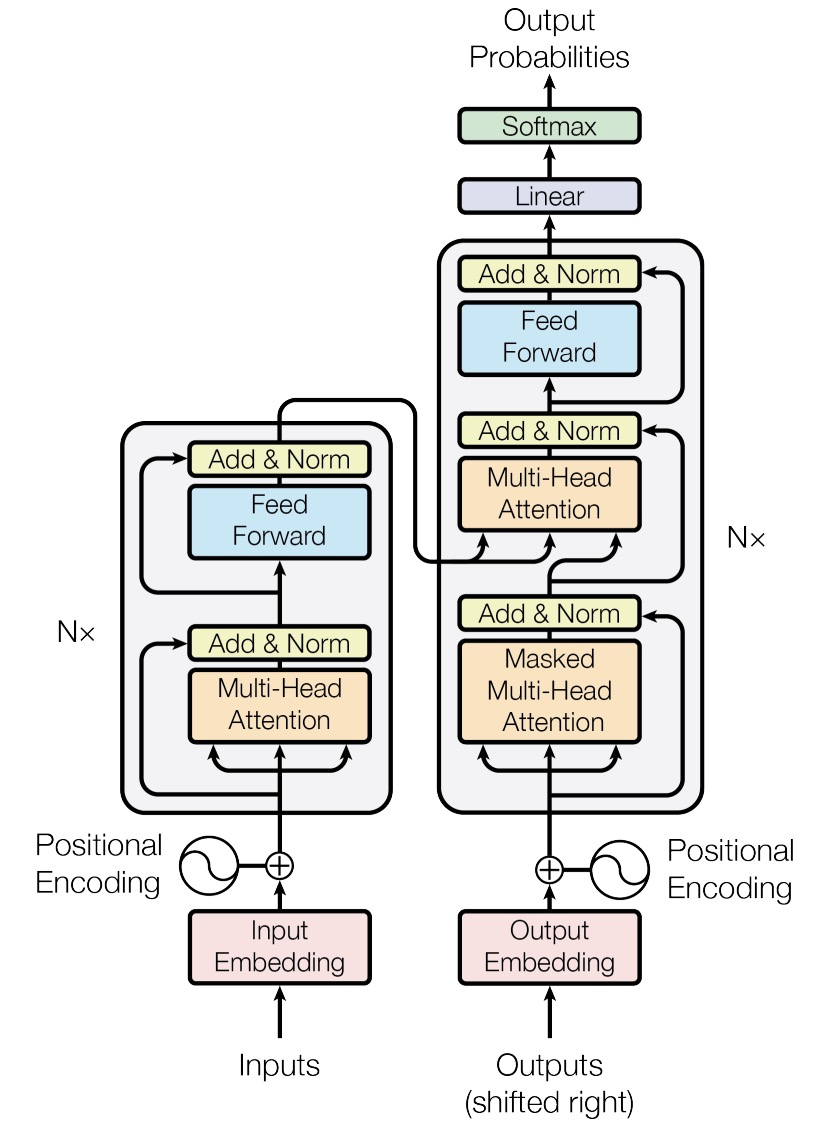
\includegraphics[width=4in]{figures/xulun/transformer.jpg}
  \caption{Transformer 结构框架\cite{vaswani2017attention}}
  \label{fig1:transformer}
  \end{figure}
Transformer 是一个基于注意力机制,特别是自注意力机制的模型,它彻底放弃了循环
神经网络(RNN)和卷积神经网络(CNN)的使用。如\figref{fig1:transformer}, 
Transformer 模型包含两个
主要部分:编码器(左边)和解码器(右边)。每个部分都由多个相同的层
堆叠而成,每层包含了自注意力机制和前馈神经网络,具体描述在\tabref{tab1:encoder}和\tabref{tab1:decoder}中。

\begin{table}[h!]
  \centering
  \small
  \begin{tabular}{lp{10cm}}
  \toprule
  \textbf{子层} & \textbf{描述} \\
  \midrule
  多头自注意力机制 & 允许模型在处理一个单词时,同时考虑句子中的其他单词。 \\
  \midrule
  前馈神经网络 & 它是一个简单的全连接网络,对每个位置的表示应用相同的线性变换。 \\
  \bottomrule
  \end{tabular}
  \caption{编码器结构描述。}
  \label{tab1:encoder}
  \end{table}
  
  \begin{table}[h!]
  \centering
  \small
  \begin{tabular}{lp{10cm}}
  \toprule
  \textbf{子层} & \textbf{描述} \\
  \midrule
  多头自注意力机制 & 与编码器中的自注意力机制类似,但有额外的掩码(Masking)来防止位置获取未来位置的信息。 \\
  \midrule
  编码器-解码器注意力 & 允许解码器关注编码器的输出。 \\
  \midrule
  前馈神经网络 & 结构与编码器的前馈神经网络一致。 \\
  \bottomrule
  \end{tabular}
  \caption{解码器结构描述。}
  \label{tab1:decoder}
  \end{table}

%\textbf{编码器}由相同的层组成。每个层包含两个子层:
%
%多头自注意力机制(Multi-Head Self-Attention):允许模型在处理一个单词时,同时考虑句子中的其他单词。
%
%\textbf{前馈神经网络}(Feed-Forward Neural Network):它是一个简单的全连接网络,对每个位置的表示应用相同的线性变换。
%解码器
%
%\textbf{解码器}同样由多个个相同的层组成,但每个层包含三个子层:
%
%\textbf{多头自注意力机制}(Multi-Head Self-Attention):与编码器中的自注意力机制类似,但有额外的掩码(Masking)来防止位置获取未来位置的信息。
%
%\textbf{编码器-解码器注意力}(Encoder-Decoder Attention):允许解码器关注编码器的输出。
%
%\textbf{前馈神经网络}(Feed-Forward Neural Network):结构跟encoder的前馈神经网络一致。

在Transformer的结构中,注意力机制扮演着核心角色。自注意力机制、缩放点积注意力和多头注意力共同构成了Transformer模型中处理序列数据的基础。

\textbf{自注意力机制(Self-Attention)}
是Transformer结构的基石,它允许模型在处理序列的每个元素时,考虑到序列中的所有其他元素。自注意力的计算公式如下:
\[ \text{Attention}(Q, K, V) = \text{softmax}\left(\frac{QK^T}{\sqrt{d_k}}\right)V \]
其中,\(Q\)、\(K\)、\(V\) 分别表示查询(Query)、键(Key)和值(Value),\(d_k\) 为键的维度。

\textbf{缩放点积注意力(Scaled Dot-Product Attention)}是自注意力机制的一种具体实现,通过缩放因子调整查询和键的点积计算。它提供了一种有效的方法来评估输入元素间的相似度。缩放点积注意力的公式为:
\[ \text{Scaled Dot-Product Attention}(Q, K, V) = \text{softmax}\left(\frac{QK^T}{\sqrt{d_k}}\right)V \]

\textbf{多头注意力(Multi-Head Attention)}
多头注意力机制通过将自注意力分解为多个``头'',在不同的表示子空间中并行执行,从而捕捉输入数据的多样化特征。多头注意力的计算公式为:
\[ \text{MultiHead}(Q, K, V) = \text{Concat}(\text{head}_1, \text{head}_2, \dots, \text{head}_h)W^O \]
其中,每个头 \(\text{head}_i\) 的计算为 \(\text{Attention}(QW_i^Q, KW_i^K, VW_i^V)\),\(W_i^Q\)、\(W_i^K\)、\(W_i^V\) 和 \(W^O\) 是模型中的可学习权重矩阵。

Transformer模型通过其创新的自注意力机制和编码器-解码器架构,为处理复杂的自然语言任务提供了强大的工具。

\subsubsection*{2) Transformer的衍生模型}

随着NLP技术的不断进步,Transformer的衍生模型,如BERT、GPT、XLNet和RoBERTa,
将Transformer结构与无监督学习结合,
可以在不同NLP任务上实现前所未有的性能,无需每个任务重新训练。
这些模型虽采用不同预训练目标和数据集,但依然可根据使用的Transformer结构分类:

\begin{equation*}
  \text{衍生模型} \left\{
      \begin{array}{l}
        \text{Encoder模型(如BERT、RoBERTa),称为自编码模型} \\ 
        \text{Decoder模型(如GPT、XLNet),称为自回归模型。}
      \end{array}
  \right.
\end{equation*}

%\begin{itemize}
%  \item Encoder模型(如BERT、RoBERTa),称为自编码(auto-encoding) Transformer模型
%  \item Decoder模型(如GPT, XLNet),称为自回归(auto-regressive) Transformer模型。
%\end{itemize}


\subsubsection*{Encoder模型}

Encoder 模型只使用 Transformer 模型中的 Encoder 模块,也被称为
自编码(auto-encoding)模型。在每个阶段,注意力层都可以访问到原始输入
句子中的所有词语,即具有``双向''注意力。
Encoder 模型通常通过破坏给定的句子(例如随机遮盖其中的词语),
然后让模型进行重构来进行预训练,最适合处理那些需要理解整个句子语义的任务,
例如句子分类、命名实体识别(词语分类)、抽取式问答。
BERT 是第一个基于 Transformer 结构的纯 Encoder 模型,它在提出
时横扫了整个 NLP 界,在流行的 GLUE 基准上超过了当时所有的最强模型。
随后的一系列工作对 BERT 的预训练目标和架构进行调整以进一步提高性能。
目前,纯 Encoder 模型依然在 NLP 行业中占据主导地位。下面简略介绍一下 
BERT 模型及它的变体RoBERTa。

\subsubsection*{BERT 模型}

BERT是基于 Transformer 架构的自然语言处理模型。它采用 Transformer 的编
码器部分来学习文本中单词或子单词之间的上下文关系。与传统的单向模型不同,
BERT 的编码器一次性读取整个单词序列,因此,虽然通常被描述为``双向''模型,
但更准确地说,它是非定向的。

BERT 的训练涉及两种主要策略:Masked LM (MLM)和Next Sentence Prediction (NSP)。
Masked LM (MLM):在输入序列中随机选择大约15\%的单词并用特殊的[MASK]标记替换,然
后模型尝试预测这些被遮盖的单词。这需要在编码器的输出顶部添加一个分类层,并且通过词嵌入矩
阵将输出向量转换为词汇量,最后使用 softmax 函数计算每个单词的概率。BERT 的损失函数
仅考虑遮盖值的预测。

Next Sentence Prediction (NSP):BERT 接受成对的句子作为输入,并学习预
测第二个句子是否逻辑上紧跟在第一个句子之后。在输入中,50\%是连续的句子对,另一
半则是随机的句子对。在输入模型之前,每个输入序列的开始位置会添加一个特殊的[CLS]标记,
每个句子的末尾添加[SEP]标记,同时引入句子嵌入和位置嵌入。为了预测第二个句子是否跟随
第一个句子,模型将[CLS]标记的输出转换为一个二维向量,并使用 softmax 计算其为连续句子的概率。

BERT 在多个基准测试上取得了显著的成绩,包括 
GLUE、SQuAD、SWAG\cite{zellers2018swag}、CLOTH\cite{xie2018large}、
DREAM\cite{sun2019dream}和 SQuAD 2.0。
BERT 通过这种方式,在理解语言的多个方面,尤其是上下文理解方面,取得了新的突破。然而,由
于其复杂的结构和依赖于大量数据的特点,BERT 在一些情况下难以解释,并且在处理特定类型的
语言数据时可能存在泛化问题。尽管如此,BERT 仍然是自然语言处理领域的一个重要里程碑,并
为后续的模型如 XLNet、RoBERTa 等奠定了基础。

\subsubsection*{RoBERTa 模型}
RoBERTa 模型代表了在深度学习和自然语言处理领域中对
BERT模型的一个重要的进化步骤。这种进化不仅基于对BERT潜力的深入挖掘,而且体
现了对预训练语言模型的深刻理解。在这一过程中,RoBERTa的开发者们采用了四个创
新和优化措施,旨在全面提升模型的性能和适应性。

首先,关于数据集的扩展和训练时长的增加,这些改变源于一个核心理念:更多的数据和
更长的训练周期能够使模型捕捉到更为复杂和微妙的语言模式。通过将数据量从BERT的16GB增
加到160GB,并将训练迭代次数从100K提升至500K,RoBERTa能够在更广泛和多样化的文本上学
习,从而提升其对于复杂语言结构的理解能力。

动态掩码的引入是RoBERTa另一个创新之处。与BERT的静态掩码不同,RoBERTa在每个epoch
中对文本采用不同的掩码模式。这种方法有效防止了模型对固定掩码模式的过度适应,从而推动模型
学习更加泛化的语言表示。具体而言,这种动态掩码策略是在训练过程中实时应用的,确保即使同一
文本在不同的训练阶段也会呈现出不同的掩码模式,增加了训练的多样性和复杂性。

此外,去除BERT中的下一个句子预测(NSP)任务也是一个关键决策。尽管NSP被设计来提高模型
对句子间关系的理解,但研究发现,在去除这一任务后,RoBERTa在多项下游任务中的表现有了显
著提升。这表明对于模型的优化,有时候减法也是一种有效的策略。

再者,RoBERTa在训练中对样本长度的处理也展示了其对复杂语言模式理解的重视。通过在训
练中始终使用全长(512个令牌)的序列,RoBERTa强化了对长距离依赖关系的学习,这对于
处理更为复杂的语言结构至关重要。

这些改进使得 RoBERTa 在多个基准测试(如 GLUE、RACE\cite{lai2017race}、SQuAD 等)
中取得了领先性能,甚
至超过了人类的表现。
综合来看,RoBERTa的这些创新和优化措施共同构成了其卓越性能的基础。通过在大规模数据
集上进行深入训练,实施动态掩码机制,精简训练任务,以及优化样本长度处理,RoBERTa不仅
巩固了BERT作为一种强大的语言模型的地位,也为后续的NLP研究提供了宝贵的参考和启示。


\subsubsection*{Decoder模型}
Decoder 模型只使用 Transformer 模型中的 Decoder 模块。在每个阶段,对
于给定的词语,注意力层只能访问句子中位于它之前的词语,即只能迭代地基于已经生
成的词语来逐个预测后面的词语,因此也被称为自回归(auto-regressive)模型。
下面就简要介绍一些常见的Decoder 模型。

\subsubsection*{GPT 模型}
GPT基于Transformer架构开发,主要使用了该架构的 Decoder 部分。
GPT 结合了 Transformer Decoder 架构和迁移学习方法,
在大量开放在线数据上进行无监督预训练,特别是在 BookCorpus 数据集上。
其预训练任务是根据上文预测下一个单词,从而使模型能够在没有限制的情况下学习语言特征。
此外,GPT 还通过微调适应各种下游任务,如文本蕴含、语义相似性、情感分析等,在包括
SNLI、MNLI、ROC、COPA 和 GLUE 等多个 NLP 基准
测试中取得了显著效果。

然而,GPT 也存在一些局限性,如高计算要求、预训练数据的不完整性及不准确性,
以及在处理高词汇变化的数据方面的泛化问题。

\subsubsection*{XLNet 模型}
XLNet的出现在自然语言处理(NLP)领域引发了显著关注,特别是它在
特定任务中相较于BERT的显著性能提升,标志着NLP模型发展的一个新阶段。这种
模型不仅继承了自回归语言模型的强大特性,同时也融合了自编码语言模型(如BERT)的优
势,创造了一种新的、更为复杂和有效的预训练机制。

XLNet的核心在于它的创新性预训练目标——排列语言模型(Permutation LM)。在
BERT中,模型预训练是通过随机选择一些单词并将其替换为[MASK]标记来进行的,
然后模型被训练来预测这些被掩盖的单词。然而,这种方法导致了一个问题:在实
际应用中,即微调(fine-tuning)阶段,输入数据中并不存在[MASK]标记,这可
能导致预训练和微调之间的不一致性。
为了解决这个问题,XLNet引入了排列语言模型。在这种模型中,对于一个给定长度
的句子,模型会考虑所有可能的单词排列组合。在每次训练迭代中,
模型会随机选择一种排列,并基于这种排列来预测单词。具体来说,对于一个句子中
的每个位置,
模型尝试预测这个位置的单词,给定在这个特定排列中它之前的所有单词。
这种方法有效地模拟了自回归(autoregressive)语言模型的特性,
同时也使模型能够在预训练中学习到上下文的全面信息。

在与BERT的比较中,XLNet的预训练机制展现出三个独特的优势:
首先,BERT通过在输入中随机遮盖某些词并预测这些词来进行训练,而
XLNet则采用了无需明显[MASK]标记的内部随机``遮盖''单词方法。这种差异使得
XLNet在预训练和微调阶段保持了更高的一致性,解决了BERT预训练与微调不一致的问题。

此外,XLNet在处理生成型任务上也表现出明显的优势。得益于其自回归特
性,XLNet能够在维持自然的从左到右的生成过程的同时,内部隐含上下文信
息,这对于生成连贯、流畅的文本尤为重要。

针对长文本的处理能力也是XLNet的一个亮点。它整合了
 Transformer XL\cite{dai2019transformer} 的技术,使
得在处理长文档类型的NLP任务时,相比BERT有着更为显著的优势。

总的来说,XLNet通过结合自回归和自编码语言模型的优势,通过其排列语言模型和注
意力掩码机制,有效地利用上下文信息。这些特性使得XLNet在多项NLP任务中,尤其是在
生成型任务和长文档处理方面,相较于BERT展现出更加卓越的性能。这种创新的预训练方法
不仅解决了先前模型的某些局限性,也为未来NLP模型的发展提供了新的方向。

%\textbf{小结}:
%在本节中,我们对一系列模型进行了深入分析。这些模型主要通过序列化训练数据来学习,
%并在常识性推理任务中表现出色。然而,研究过程揭示了这些模型的一些显著不足。
%首先,即使是经过大规模数据训练的预训练模型,也难以全面掌握全部常识性
%知识\cite{lin2020birds,peng2022copen}。实验结果表明,所有预训练
%语言模型在零样本探测任务上均优于随机猜测,这证明了它们在概念性知识获取方面的潜力。
%然而,即便经过微调,这些模型的准确率仍未能达到人类水平\cite{peng2022copen}。因此,
%探索如何将更多的常识性知识整合到现有模型中,以增强其概念性知识推理能力,成为了一个
%关键的研究方向。

%与此同时,我们也注意到,尽管大型预训练语言模型在NLP领域取得了显著进展并
%在现实世界中得到了广泛应用,
%但它们在处理领域外数据、抵御对抗性攻击\cite{mccoy2019right,jin2020bert}以及应对输入的微
%小扰动\cite{ebrahimi2018hotflip,belinkov2018synthetic}方面仍显脆弱。这些局限性
%可能会阻碍这些模型在实际环境中的安全部署,并影响用户对NLP模型的信任度。为了应对这些
%挑战,语言技术领域的研究者们正加大力度,旨在深入理解并解决这些鲁棒性问题。
%在下一节中,我们将进一步讨论自然语言推理任务中模型鲁棒性的相关研究。

\subsubsection{推理模型鲁棒性研究}
\label{sec1:robustness}
上一小节是我对我所研究的相关的推理方法的介绍,尽管大型预训练语言模型在NLP
领域取得了显著进展并
在现实世界中得到了广泛应用,
但它们在处理领域外数据、抵御对抗性攻击\cite{mccoy2019right,jin2020bert}以及应对输入的微
小扰动\cite{ebrahimi2018hotflip,belinkov2018synthetic}方面仍显脆弱。这些局限性
可能会阻碍这些模型在实际环境中的安全部署,并影响用户对NLP模型的信任度。为了应对这些
挑战,语言技术领域的研究者们正加大力度,旨在深入理解并解决这些鲁棒性问题。
在这一节中,我们将进一步讨论自然语言推理任务中模型鲁棒性的相关研究。
%接下来是对这些模型在具体任务上的鲁棒性的探究的相关工作,
包括模型的鲁棒性的测试和提高模型鲁棒性的相关方法。

\subsubsection*{1. 鲁棒性的定义和测试方法}

Wang等人(2022)\cite{wang2022measure}对模型的鲁棒性进行了定义:

\begin{definition}[鲁棒性]
在自然语言处理(NLP)模型中,\textbf{鲁棒性}指的是模型在面对不同分布的测试数据时保持性能的能力。
具体来说,对于一个输入 $x$ 和它的正确标签 $y$,对于一个在 $(x, y) \sim D$ 上训练的模型 
$f$ 及其对 $x$ 的预测 $f(x)$,鲁棒性是通过模型在测试数据 
$(x', y') \sim D'$(可能与 $D$ 分布不同)上的表现来衡量的。
通常使用诸如鲁棒准确率这样的指标来量化鲁棒性,
定义为 $E_{(x', y') \sim D'}[f(x') = y']$。
\end{definition}

在探讨模型鲁棒性的文献中,可以粗略地将他们分为两类:对抗性攻击下的鲁棒性和分布偏移下的鲁棒性。
对抗性鲁棒性关注在输入 $x$ 周围创建微小扰动 $\delta$ 形成 $x'$ 时模型的表现,
而分布偏移鲁棒性关注在自然发生的不同分布上的模型表现。
这些分类共同探讨 $D'$ 是合成分布偏移(如对抗性攻击)还是自然分布偏移。

\textbf{对抗性攻击下的鲁棒性}:
对抗性鲁棒性的研究主要集中在模型对输入的微小扰动($\delta$)的反应上,
即在原始输入 $x$ 周围引入扰动,形成 $x'$,并观察模型的响应。这类攻击通常通过添加
对人类几乎不可察觉的噪声,以欺骗模型做出错误判断。这种策略最初在计算
机视觉领域被广泛研究\cite{szegedy2014intriguing,goodfellow2014explaining},
随后扩展到自然语言处理(NLP)领域\cite{Marco2020acl,tan2020s,schwinn2023exploring,boucher2022bad},
凸显了对NLP模型进行全面鲁棒性评估的重要性。

\textbf{分布偏移下的鲁棒性}:
与之相对,分布偏移下的鲁棒性关注模型在不同自然分布的数据上的表现。
这类研究反映了现实世界数据多样性和复杂性的影响,如语法错误、方言、
语言差异等因素\cite{blodgett2016demographic, demszky2021learning},以及
同一任务在不同领域的新数据集上的表现。

%对于NLP模型的鲁棒性,已有多项工作尝试理解和测量其在不同任务中的表现
%\cite{tu2020empirical,sagawa2020investigation,geirhos2020shortcut}
%特别是在自然语言推理(Natural Language Inference, NLI)任务中,
%研究者们通过对错误分类样本的分析,确定了导致错误的常见原因,
%并据此构建压力测试集。
CheckList\cite{Marco2020acl}是一个结合了对抗性攻击和分布偏移下鲁棒性测试的方法论。
它借鉴软件工程中的``黑盒测试''方法,重点评估NLP模型在不同输入变化下的表现。这一方法论包括三
个核心部分:功能评估、测试方法和测试用例生成。

1)功能评估:此部分更多关注模型在处理各种NLP任务(如语义角色标注、命名实体识别等)时的能力,
为后续的鲁棒性测试奠定基础。

2)测试方法和测试用例:这里包括对抗性攻击下的鲁棒性和分布偏移下的鲁棒性两个方面。
对于前者,CheckList通过模拟对抗攻击中的微小变化或扰动(如情感分析中的句子轻微修改),
评估模型的反应\cite{goodfellow2014explaining}。它通过不变性测试(INT)和定向期望测试(DIR)等方法,
检验模型在处理对抗性攻击下的鲁棒性(如语法结构变化、情感强度变化)时的稳定性。同时在分布偏移的鲁棒性的测试中,
CheckList通过模板方法简化了大量有效测试用例的创建。
例如,可以创建一个模板``我\{NEGATION\}\{POS\_VERB\}这个\{OBJECT\}'',
并通过不同的词语组合生成多个测试句子,如``我不喜欢这个电影'',来评估模型对否定构造的处理能力。这些例子的主题和分布与原来的测试集已经完全不同。

总结来说,CheckList为NLP领域提供了一个全面的框架,
用于评估和提升模型在面对对抗性攻击和分布偏移时的鲁棒性。
这不仅有助于揭示模型的潜在薄弱环节,也为提高模型的整体鲁棒性提供了实践指导。


%除了CheckList以外,还有很多的压力测试数据集用来测试模型的鲁棒性,下面本文要介绍四个
%常识性推理模型比较常用的压力测试集:

%\textbf{Stress Test数据集}:
%在2018年,Naik及其团队推出了一种创新方法\cite{naik2018stress}来评估自然语言推理(NLI)
%模型的鲁棒性,被称为``Stress Test''。这个方法核心在于探索NLI模型如何应对语言的多样性和复杂性,
%特别是在真实推理能力方面。他们设计了一系列实验,仔细检验了模型在理解\textit{词汇重叠}、\textit{处理否定句}、
%\textit{识别反义词}、\textit{执行数值推理},以及\textit{应对长度不匹配}和\textit{语法错误的句子}等方面的能力。
%此外,这个测试还考察了模型在处理现实世界知识和模糊情境时的表现。
%这种多维度的测试不仅展示了NLI模型在复杂语言处理上的潜力,
%同时也揭示了它们的局限,为未来的研究和改进提供了方向。
%
%\textbf{HANs数据集}:
%在NLI领域的深入研究中,McCoy和同事们在2019年引入了HANs数据集\cite{mccoy2019right},
%致力于解决NLI模型过分依赖简单句法启发式的问题。这个数据集着重检验了模型是否只是依赖于词汇重叠、
%子序列和成分等表面特征来做出判断。研究者们精心设计了一系列模板,每个模板都旨在测试
%特定的启发式策略。这种方法确保了每个测试案例既具有合理性又富有挑战性。HANs数据
%集的发现表明,即使是先进的模型如BERT,在这些句法启发式上也可能表现不佳,揭示了
%这些模型在深层语言理解方面仍有很大的提升空间。
%
%\textbf{Adversarial-NLI(ANLI)数据集}:
%2020年,Nie及其团队引入了Adversarial-NLI(ANLI)数据集\cite{nie2020adversarial},
%标志着NLI领域的一次重大进步。ANLI采用了一种迭代的、对抗性的人机共同循环程序,
%不断地推进数据集的演进并带来新的挑战。在构建这个数据集的过程中,研究团队邀请了非专
%家的人类注释者基于给定的上下文来编写假设,随后使用这些假设的模型预测来引导更多的数据
%收集。这个过程的目的在于发掘并利用模型的弱点。ANLI的创新之处在于其动态和对抗性质,使
%其能够持续适应并挑战最先进的自然语言理解(自然语言推理)模型。这个数据集不仅测试了模型在不同来源
%和上下文中的适应性,而且还推动了自然语言推理领域的界限。
%
%\textbf{Generated FEVER Test数据集}:
%2019年,Schuster及其团队引入了Generated FEVER Test\cite{schuster2019towards},
%这是一个旨在解决事实验证模型中偏见问题的数据集。它检验了在FEVER数据集上训练的
%模型是否仅依赖于索赔中的表面线索而非进行基于证据的深入事实验证。通过创新地构建对称测试集,
%包含原始索赔-证据对及其对立对,Generated FEVER Test迫使模型超越表面线索,
%转向更深入的推理和证据评估。此外,数据集还包含一种重新加权方法,用于调整实例重要性,
%平衡n-gram与标签之间的相关性,特别是针对与特定标签紧密关联的短语。这项工作不仅增加了事
%实验证模型的挑战性,也在创建公平无偏见的数据集方面迈出了重要步伐,显示了模型在处理复杂
%和需要深层理解的情境时的性能下降,从而强调了提升模型在理解和验证事实方面能力的必要性。
%
%这些研究展示了在自然语言处理中,尤其是在自然语言推理任务上,
%针对分布偏移和模型鲁棒性的持续探索的重要性。未来的研究可能会更深
%入地探讨如何系统地识别和应对这些挑战,以及如何整合这些策略以提高NLP系统
%在现实世界应用中的公平性和有效性。
%
\subsubsection*{2. 增强模型鲁棒性的方法}
在自然语言推理领域,增强模型的鲁棒性是一个关键目标。
我们可以将这些增强方法分为两个主要类别:数据增强方法和基于模型和训练方案的方法。

1) 数据增强,作为优化大规模神经网络模型性能的核心策略,
在自然语言处理领域的应用尤为关键。本文概述了几种主要的文本数据增强技术及其在学术研究中的应用,展示了它们如何为自然语言推理任务带来显著的性能提升。

\textbf{回译(Back-translation)}\cite{sennrich2016improving,edunov2018understanding,xie2020unsupervised}:
通过将文本从一种语言翻译到另一种语言,再翻译回原语言,创造出文本的新变体,从而增加数据的多样性。

\textbf{c-BERT词替换}\cite{wu2019conditional}:
运用BERT模型来识别并替换文本中的关键词汇,生成文本的新版本,以此来丰富语料库。

\textbf{混合(Mixup)}\cite{guo2019augmenting,chen2020mixtext}:
通过在不同文本样本之间进行线性组合,创造全新的文本实例。

\textbf{截断(Cutoff)}\cite{shen2020simple}:
分为两类:Token截断,即随机选取Token,将对应Token的嵌入整行置零;特征截断,
即随机选取嵌入的特征,将所选特征维度整列置零。

2) 基于模型和训练方案的方法,一般指的是调整模型结构来增强模型在自然语言推理任务当中的鲁棒性。
最常用的方法是\textbf{对抗性训练}\cite{zhu2019freelb,jiang2020smart},
这种方法通过在词嵌入层引入微小的扰动,合成附加样本,提高模型对异常输入的鲁棒性。
该方法通过梯度反传生成对抗性扰动,并加到原始嵌入矩阵上,产生增强样本,
通常应用于有监督训练场景。

在Qu(2020年)\cite{qu2020coda}的研究中,通过比较这些模型增强技术
在RoBERTa模型上处理自然语言推理任务(MNLI)的效果,发现回译和对抗性训练在提升模型
性能方面效果显著,明显优于c-BERT、混合和截断技术。因此,将回译作为自然语言推理任务中的一
种强有力的基准进行数据增强方法比较,是一种合理的策略。这些研究成果不仅强调了数据增强在提
升模型性能方面的重要性,还为选择适当的数据增强策略提供了宝贵的指导。

\subsubsection{推理模型可解释性研究}
\label{sec1:interpretability}
%上一小节是对模型鲁棒性的一些发现和增强的研究,
%但是我们可以看出即使是覆盖面很广的Checklist也只能说明模型在某些方面,
%比如``semantic role labeling'',``role labeling''或者对抗攻击下的鲁棒性测试,
%但是无法说明到底是什么原因导致的我们可以看出即使是覆盖面很广的Checklist也只能说明模型在某些方面的能力是不足的
%这种解释并不具体,而且里面还涉及人工书写templete,成本较高。

%其他的针对模型不鲁棒的原因的探索还有hypothesis-only 
%和 attention map,hypothesis-only是为了探究分类或者多项选择模型在没有前提只有选项的情况下能否做出正确推理的一种评估模型从
%只看选项这种模式中获益的程度来评估模型是不是没有学习到推理能力,就像我们常说的``三短一长选一长''这种偏差,这种方式从一定程度上说明了问题,
%但是并不完全严谨,因为毕竟模型的真实输入是包含题目的前提的,测试的时候输入的改变可能引起推理方式的改变,
%这种变化不能完全说明原来的推理模式是完全不关注推理能力而是只关注spurious features的。这个方式的另一个弊端就是必须复现模型,如果是模型比较庞大但是资源有限的情况下就很难进行分析。
%
%attention map跟前两种方法相比是一种更直接的white-box的方式,
%大家可以根据attention的权重来分析模型的表现,这看似最科学的方法却已经被证明并不可靠,attention的权重
%并不完全具有可解释性的含义

%所以如何更好的解释模型的表现,比如不鲁棒,就成了一个很重要的课题。

\subsubsection*{1. 模型鲁棒性的限制}
在前一节对模型鲁棒性的深入探讨中,我们注意到这些研究虽然关注了特定任务
(如``语义角色标注''和对抗攻击)下的模型表现,但未能充分解释模型鲁棒性差背后的推理机制\cite{hendrycks2020pretrained}。
例如,Checklist方法\cite{Marco2020acl}
在评估模型某些方面的能力时,未能深入挖掘导致模型不足的根本原因。

\subsubsection*{2. 短路行为的识别及其影响}
这引出了一个关键问题:模型在处理复杂任务时是否真正进行深度推理,
或仅仅是依赖于数据中的简单模式或偏差。这种现象被称为``短路行为''(short-circuit behavior)\cite{huangacombating},
在自然语言推理(NLI)任务中表现尤为明显。McCoy等人(2019)\cite{mccoy2019right}的研究表明,
在NLI任务中,模型可能倾向于依赖关键词或句子结构,而忽略两个句子之间真正的逻辑关系。

\subsubsection*{3. 探索短路行为的方法}

%\Shan{attention map这里有个图, hypothesis only这里加个例子}
为了深入分析和量化机器学习模型中的短路行为,研究人员开发
了``仅假设''测试(``hypothesis-only'')\cite{gururangan2018annotation}和
注意力图(attention map)\cite{vig2019multiscale}这两种方法。这些方法都旨在评
估在缺乏充分上下文信息的情况下,模型是否
过度依赖于选项本身的特征。

1) 仅假设测试

``仅假设''测试的核心思想是检验模型在仅凭假设(即问题或选项本身)的情况下的表现。
这种测试通常用于评估自然语言理解模型。在这种测试中,模型只被提供假设部分,而没
有相应的前提或上下文信息,比如在 \secref{sec1:challenge} 中提到的SNLI的例子,只提供假设
``A man is pushing a baby carriage'' 而不提供前提,让模型猜测前提跟假设之间的关系。
从人的角度来看,
解决这个问题是不可能的,因为问题本身有缺陷,很难做出选择,但是如果模型依然做出跟有前提时一致的结果,
研究者就可以判断模型可能过度依赖于假设中的某些关键词或短语,而忽
略了理解整体意义所必需的上下文。

这种方法的优点在于它能够揭示模型可能的短路行为,即模型可能仅凭借假设
中的关键信息做出判断,而不是进行全面的理解。然而,它的一个限制是无法完全反映
模型在处理真实场景时的推理模式。在现实世界的任务中,模型通常需要综合考虑全面的上下文信息。

2)注意力图

注意力机制是深度学习中的一种重要技术,它帮助模
型聚焦于输入数据的关键部分。注意力图是一种可视化工具,它展示
了模型在做出决策时对不同输入部分的关注程度。通过观察这些图,研究者
和开发者可以更直观地理解模型的决策过程,识别模型关注的是哪些信息。

尽管注意力图提供了一个看似直观的方式来解释模型的行为,但其可靠性
和解释性并非总是确定的。研究表明,即使是通过注意力机制突出显示的部分,也不
一定准确地反映了模型决策的真正依据\cite{jain2019attention}。这意味着,虽然
注意力图为我们提供了洞察模型决策过程的一个窗口,但它并不能完全代表模型的内部工作机制。

总的来说,这两种方法都为理解和评估模型提供了有价值的工具,但它们各有局限性。
理解这些方法的优缺点有助于更全面地评估机器学习模型的行为和决策过程。

%为了更好地理解和量化短路行为,``仅假设''测试(``hypothesis-only'')\cite{gururangan2018annotation}
%和注意力图(attention map)\cite{vig2019multiscale}这两种方法应运而生。
%它们旨在评估模型是否在缺乏完整上下文的情况下,过度依赖于选项本身。
%然而,``仅假设''测试虽然揭示了模型可能的短路行为,但并不能完全反映模型在真实场景下的推理模式。
%同样,尽管注意力图为理解模型的决策过程提供了直观的白盒视角,
%但它的可解释性并非总是可靠\cite{jain2019attention}。

\subsubsection*{4. 数据集偏差对模型性能的影响}
此外,模型的鲁棒性失败有时也可以归因于数据集偏差。
例如,Lewis等人(2021)\cite{lewis2021question}指出,问答模型在训练和测试数据重叠显著的情况下表现更差,
凸显了数据集在模型泛化能力评估中的重要性。在自然语言推理任务中,数据集偏差同样影响
模型性能的准确估计\cite{bras2020adversarial}。

综上所述,为了深入理解和解释模型的推理能力,特别是在面对短路行为时,
我们需要开发更精确的测试方法和分析工具。这不仅将提高模型的透明度和可靠性,
而且将优化它们在复杂真实世界任务中的应用。


%transformer 非常值得参考
%https://transformers.run/back/transformer/
%
%https://zhuanlan.zhihu.com/p/70257427
%
%https://towardsdatascience.com/what-is-xlnet-and-why-it-outperforms-bert-8d8fce710335
%https://www.jianshu.com/p/7677e1a5813c
%
%首先介绍AI 五个范式的变化,然后在五个范式变化中常识性推理相关的研究的相应变化。主要是方法的变化
%https://zhuanlan.zhihu.com/p/615507319
%
%常识性推理的现有研究:综述当前关于常识性推理的研究,包括主要的理论框架、模型和实现方法。
%
%
%可解释AI的相关研究:探讨可解释人工智能的相关工作,特别是那些与常识性推理相关的研究。
%
%
%稳定性在AI系统中的研究:分析稳定性在人工智能系统中的作用,特别是在常识性推理方面的应用。
%
%技术和方法的比较:比较现有技术和方法在处理可解释性和稳定性方面的优势和局限性。
%
%研究差距和挑战:识别当前研究中的空白和挑战,为您的研究定位。
\fi

\subsection{研究内容和贡献}
%我的研究围绕常识性推理领域中的三个重要挑战(\secref{sec1:challenge}中描述)展开:
%第一,提升模型常识性推理能力的挑战;第二,
%解析模型鲁棒性不足的原因的挑战;第三,增强常识性推理模型鲁棒性的挑战。
%针对这些挑战,我们深入分析了现有研究(如\secref{sec1:related}所述),
%特别关注了推理模型和方法(\secref{sec1:approachs})、
%常识性推理模型鲁棒性(\secref{sec1:robustness})
%以及常识性推理模型可解释性(\secref{sec1:interpretability})方面的研究进展。
%下面我将介绍针对这三个挑战我的主要研究内容和贡献。整体结构在\figref{fig1:structure}中表示。
我的研究重点围绕常识性推理领域中的三个关键挑战展开,
如第一节(见 \secref{sec1:challenge})所述。首先是提高模型在常
识性推理方面的能力,其次是解析模型在鲁棒性方面的不足的原因,以及
最后一个挑战,即增强常识性推理模型的鲁棒性。

在下文中,我将介绍我在应对这三大挑战方面的主要研究内容及研究的贡献。
我的研究的整体结构和逻辑框架在图 \figref{fig1:structure} 中有清晰的展示。

\begin{figure}[th]
  \centering\includegraphics[width=5in]{figures/xulun/structure.eps}
  \caption{研究内容的整体结构。}
  \label{fig1:structure}
  \end{figure}


\subsubsection{基于知识增强的常识性推理研究}

\subsubsection*{1. 研究内容}
在应对常识推理任务的首个挑战,即增强模型在常识性推理方面的能力时,
我们的研究聚焦于目前领先的神经网络方法,比如BERT。我们深入分析了这些方法的应用。
虽然神经网络在常识推理任务中展现出强大的性能,
但根据Lin等人的研究\cite{lin2020birds,peng2022copen},在处理常识性知识时,
这些方法仍有提升的空间,特别是在精确把握和表达这些知识时。

为了在常识性推理领域实现进一步的突破,我们选择了一个极具挑战性的任务:
预测叙事故事的结尾。这一任务的设计灵感来源于早期关于故事理解的研究\cite{meehan1977tale},
并随后演化为预测故事中可能发生事件的任务\cite{chambers2008unsupervised}。我们的研究在ROC
故事填空测试数据集\cite{mostafazadeh2016corpus}上进行了实验,
该数据集特别设计用于评估这种预测能力,它要求参与者从两个备选结局中
选择一个最符合四句话故事情境的结局。通过这些实验,我们旨在深入探究并提升模型在
理解和预测故事结尾方面的能力。

相关研究的初步探索集中在如何计算候选结局与故事情境句子之间的语义相似度。
这通常包括对故事句子进行多维度表征,
例如通过句子中词向量的聚合\cite{mikolov2013distributed},应用
sentence2vec\cite{kiros2015skip},DSSM\cite{huang2013learning}或采
用其他创新特征\cite{schwartz2017story}。最新的方法趋向于采用双层结构:
一是利用LSTM\cite{hochreiter1997long},GPT\cite{radford2018improving}或
BERT\cite{devlin2018bert}等预训练语言模型构建句子的深层表征;
二是在ROC数据集上对分类模型进行微调,形成一个全面的故事情境表征。

在此基础上,我们提出了一种新颖的方法,专注于识别和优化故事中的关键概念。
我们发现,在故事推理过程中,将注意力集中在特定关键概念上,而非全部词汇,可以
更有效地指引至正确的结局。因此,我们设计了一种策略,在利用语言模型之前,通过
突出重要概念并降低不重要概念的影响力,来简化句子。这种方法有效地降低了模型处理
的噪音,并使其更专注于捕捉故事的核心信息。这些经过优化的句子被视为事件和概念的集
合,而这些概念在ConceptNet\cite{speer2017conceptnet}——一个全面覆盖常识推理所
需知识的开放领域知识图谱中有所定义。

此外,我们不仅注重于句子内概念的序列化处理,而且还将结构化的常识知识整合进
句子表征中。通过融入预训练的概念嵌入到故事句子表征中,我们能够更准确地捕捉故事情
境与结局之间的关键概念联系。例如,通过\textit{CapableOf}和\textit{MotivatedBy}这样
的预定义关系,我们能够揭示``long for break''与``have a rest''之间的联系,从而在故事中实现更精准的推断。

值得强调的是,我们的方法在ROC故事填空测试数据集上展示了卓越的性能。
尽管现有研究已在故事结局预测任务上取得了一定的进展,但这些成果主要集中
在原始数据集的验证部分。为了确保我们的方法的有效性和泛化能力,我们避免了使
用原始数据集的验证集,而是特意构建了一个新的训练集,该训练集与测试集不共享统
计特征。这种严谨的实验设计使我们的评估结果更加可靠,同时也证明了我们所提出方法
在提高故事理解和预测能力方面的显著效果。

\subsubsection*{2. 主要贡献}

本研究在常识性推理领域引入了一种创新且有效的方法论。我们实施
了一种精心设计的句子简化策略,专注于故事中关键概念的提炼。这种方法不仅
降低了模型处理的复杂性,而且通过集中处理核心信息,极大地提高了模型捕捉
故事情节的精准度。通过将这些精化的概念与ConceptNet数据库中的丰富结构化
知识结合,我们在故事推理任务的准确性上实现了显著的提升。
%这种方法的效果不
%仅体现在故事结局预测的准确率上,更在于其在增强模型处理故事中常识性知识的
%能力方面取得的重大进步。

在实验方法上,我们通过精心筛选和优化的训练数据集来确保了评估的公正性和准
确性。这种方法学的应用不仅提升了故事结局预测的性能,还为常识性推理中结
构化知识的有效运用提供了新的视角。本研究的贡献不仅在于推动了常识性推理领域
的发展,也为未来相关领域的研究提供了宝贵的方法和见解。

\subsubsection{推理模型鲁棒性不足的可解释性分析}
\subsubsection*{1. 研究内容}

从\figref{fig1:structure}中可见,挑战二和挑战三均源于同一现象:推理模型
的鲁棒性不足。尽管多种推理模型在常识性推理任务上取得了显著的成就,但它们在处理
对抗性数据或与训练环境不同的场景时表现出了鲁棒性不足的缺陷。

在探究推理模型鲁棒性不足的原因时,关键在于分析模型处理信息的方法和重点。
研究表明,模型可能过度依赖数据的某些特定结构元素,例如,
在处理\textit{前提}和\textit{假设}的关系时,
它们可能只关注\textit{假设}部分,而忽略了前提与假设之间的逻辑联系\cite{naik2018stress,mccoy2019right,schuster2019towards,nie2020adversarial}。
这揭示出模型可能主要学习数据中的统计偏差,也就是所谓的偏见线索(bias cues)或者
虚假线索(spurious cues)。

对这一现象出现的原因一种假设是数据集的构建方式存在偏见。模型往往学习特定于
数据集的简化规则或者偏见,而非解决问题的通用策略。例如,在自然语言处理中,如
果一个数据集中的大多数``正确''样本都包含某个特定词汇,模型可能仅依赖这个词
汇做出判断,而未深入理解句子间的逻辑关系。这种简化学习方式导致模型在面对
结构或上下文有差异的新数据时变得脆弱,无法有效适应或正确解释。如果这种线索刚好在\textit{假设}部分,
那可能就会造成模型只关注\textit{假设}部分。

为验证模型可能过度关注数据特定结构元素的假设,研究者们开发了``仅假设''测试\cite{gururangan2018annotation}和
注意力图\cite{vig2019multiscale}
这两种方法来分析和量化这一现象。尽管这些工具在解析和评估模型行为方面
发挥着关键作用,它们在深入探讨数据偏见如何影响模型核心机制方面存在局限性。
因此,深入研究数据偏见对模型机制的具体影响已成为一个紧迫且重要的研究课题。

对此问题,我们设计了两种测试框架来应对这一挑战。第一种是宏观层面的测试框架,基于统计特
征来进行评估;第二种则是微观层面的详细统计分析框架。

%从\figref{fig1:structure}中我们可以看出挑战二和挑战三都来源一个现象,
%就是推理模型的鲁棒性差这个现象
%虽然很多推理模型在众多常识性推理任务上取得了显著成就,
%但是它们在处理对抗性数据或不同于训练环境的场景时仍显脆弱。
%这种局限性通常源于模型对数据集中特定模式的过度依赖,而非深入理解问题本
%质\cite{naik2018stress,mccoy2019right,schuster2019towards,nie2020adversarial}。

%虽然已有一些研究努力揭示了模型学习过程中的
%一些不足,如CheckList\cite{},但对于模型学习到的具体内容还需更加精细和系统的分析。
%因此,我们提出了两种测试框架:一种是宏观层面上基于统计特征的测试框架,
%另一种则是微观层面的详细统计分析框架。

%在解决第三个挑战时,即深入探讨常识性推理模型鲁棒性不足的根本原因,
%正如\ref{sec1:interpretability}小节所述,
%我们发现模型鲁棒性的评估过程不仅揭示了模型的潜在不足,如通过工具Checklist等所指出的,
%而且还暴露了模型可能倾向于学习短路(short-circuits)或虚假特征(spurious features)。
%然而,这些评估方法虽然提供了宝贵的见解,但在深入探究模型确切学到了什么方面,
%尚存在一定的探索空间。这意味着,虽然已有一些研究努力揭示了模型学习过程中的
%一些特征,但对于模型学习到的具体内容和其背后的复杂动态,还需更加精细和系统的分析。
%因此,我们提出了两种测试框架:一种是宏观层面上基于统计特征的测试框架,
%另一种则是微观层面的详细统计分析框架。

\subsubsection*{宏观层面的统计特征测试框架}

在宏观层面,我们的研究主要集中于分析自然语言推理任务中的虚假线索问题。
我们注意到,尽管人类在处理这类问题时通常会分析问题前提与假设之间的逻辑关系,
许多NLP模型却倾向于主要关注假设部分,忽略了深入的逻辑分析。这种现象往往是由
于数据集中的人为偏差所引起。

在评测和分析数据集方面,我们提出了一种基于统计学线索发现的方法。
这个方法首先应用统计学公式来拟合``仅假设''模型,以便识别数据集中最具代表
性的统计特征。这种方法不仅揭示了数据集中的偏见和虚假线索,还为我们提供了一
种衡量数据集质量的有效工具。

进一步地,我们设计了一种多次采样测试方法,将测试数据划分为简单和困
难两类。这种划分旨在衡量模型在处理复杂推理任务时的真实能力,同时量
化比较简单和困难子集之间的性能差异。通过这种方法,我们能够评估模型是
否过度依赖于数据中的简单线索,从而揭示模型在不同情境下的潜在弱点。

此外,这种宏观评估方法不仅揭示了数据集的质量,还为我们提供了关于模型在
逻辑推理能力上的深刻见解。这种方法的应用有助于我们理解模型在解决自然语言推理任务时的
潜在限制,并指导我们如何改进模型以提高其泛化能力和鲁棒性。

\subsubsection*{微观层面的统计分析框架}
在更细致的层面,我们采用了微观统计分析框架--ICQ(``I-see-cue'',即``我发现线索'')框架,
这一工具旨在揭示和分析自然语言推理任务中数据集和模型的偏见性线索。ICQ框架的
应用分为两个主要领域:一是探索数据集中潜藏的偏见线索;二是评估偏见线索对模型性能的影响。

在数据集分析方面,ICQ框架旨在识别可能在数据集制作过程中不经意间引入的偏见性线索。
这些线索可能表现为特定词汇的使用、独特的短语结构或特别的语境模式。通过分析
这些线索的词汇频率、共现模式以及它们与目标标签的关联性,ICQ揭示了潜在的误
导源,增强了我们对数据集如何影响模型预测的理解。

在模型分析方面,ICQ重点分析自然语言推理模型如何在训练过程中学习和依赖这些线
索。我们采用了准确性测试和分布测试两种方法,以全面了解模型对数据集中
的偏见性线索的敏感度。准确性测试揭示了模型在处理包含或缺失特定线索的数
据样本时的表现,从而展示了模型对这些偏见性线索的依赖程度。而分布测试则
通过可视化分析,探究了特定特征分布的变化如何影响模型的预测性能,为我们提供了更直观的理解。

将这两种测试方法结合,ICQ框架为我们提供了一个全面的视角,以分析和评估
模型在学习和反应偏见性线索方面的行为。这种综合性的分析方法不仅增强了我们
对模型行为的认识,还促使我们在发现偏见时采取相应措施,以提高模型在处理具有潜
在偏见的复杂数据时的鲁棒性和推理能力。这对于构建更加公正、高效的自然语言推理系统具有重要意义。

%在更细致的层面,我们采用了微观统计分析框架,该框架结合模型的表现对测试集进行多维特征划分。
%通过这种方法,我们能够对模型在各个特征上的准确性测试和分布测试的表现进行深入分析,
%进而解释模型是否对某些分布不均衡的特征过于敏感。此外,我们还开发了一种可视化工具,
%以直观地展示这些测试结果,帮助研究人员更有效地识别和理解模型性能差异的潜在原因。

%\subsubsection*{方法和应用}

%通过深入分析神经网络模型在自然语言推理、论证分析和常识推理等任务中的表现,
%我们注意到这些模型可能倾向于利用数据集中的表面统计模式来预测正确答案。例如,
%在SNLI数据集中的多项选择问题中,模型可能仅依赖假设就能找到正确答案,这揭示了数据
%集中手工制作假设的人为误差。
%
%为应对这些问题,我们提出了ICQ(``I-see-cue'',即``我看到线索'')框架,这
%是一个灵活的统计分析工具,用于识别多项选择自然语言推理数据集中的简单但有影响力的
%线索。与传统方法相比,ICQ无需额外的测试案例即可识别自然语言推理数据集中的偏见。它采用黑
%盒测试方法,不仅评估模型如何利用这些偏见,而且为理解自然语言推理任务中的偏见提供了全面的视角。
%
%我们在各种自然语言推理数据集上部署ICQ,探测了模型在训练期间可能学到的线索。ICQ有
%助于深入理解模型如何学习潜在偏见,并为其实际应用提供了宝贵的见解。

\subsubsection*{2. 主要贡献}

本研究的主要贡献在于开发了这两种创新的分析框架,
它们为深入理解并提升常识性推理模型的鲁棒性提供了新的视角。
通过宏观和微观的方法,我们能够全面评估模型在面对复杂数据时的行为,
特别是在识别和处理潜在的虚假特征方面。这不仅有助于揭示模型可能的薄弱环节,
也促进了对模型学习机制的深入理解,为未来设计更为健壮和可解释的人工智能系统奠定了基础。

本研究的主要贡献在于开发了这两种创新的分析框架,
它们为深入理解常识性推理模型的鲁棒性不足的现象提供了新的视角。
%本研究的主要贡献在于深度探究和分析自然语言理解(自然语言推理)任务中的数据集和模型之间的复杂相互作用,特别是通过宏观和微观角度的综合分析,揭示了数据集中的偏见性线索及其对模型行为的影响。

在宏观层面,我们分析了自然语言推理数据集的结构和内容,探究了如何在数据
集创建过程中可能不经意间引入的偏见性线索。通过识别这些数据集中的特
定词汇使用、独特的短语结构,我们深入理解了这些偏见是如何形成的,以及它们可
能如何导向模型的预测。

微观层面的分析则集中在应用ICQ框架,一个专为分析模型对数据集中偏见性线索
的响应而设计的工具。通过ICQ,我们进行了准确性测试和分布测试,深入探讨了模型
如何在训练过程中对这些线索产生依赖,以及这种依赖如何影响模型的推理能力和整体性
能。ICQ的应用使我们能够更细致地观察模型对特定特征分布变化的敏感性,为理解模型行为提
供了更加丰富和直观的视角。

这两个层面的分析相辅相成,它们共同揭示了自然语言推理任务中数据集与模型之间的复杂关系,尤其
是在理解和处理偏见性问题时。本研究不仅为理解自然语言推理系统中的数据集和模型交互提供了深
入的见解,也为构建更加公平、有效且鲁棒的自然语言推理系统提供了实践上的指导。这些贡献对于未
来在该领域的研究和应用具有重要的意义,为改进数据集质量和提升模型处理能力提供了支持。

\subsubsection{提升常识性推理模型鲁棒性的数据增强策略}

\subsubsection*{1. 研究内容}
%在应对常识性推理模型鲁棒性不足的挑战时,
%我们在\secref{sec1:robustness}中探讨了模型鲁棒性的定义和测试方法。
%研究指出,尽管神经网络模型在多个任务上表现出色,其鲁棒性的不足却严重限制了模型的泛化能力。
%并且在上一节对模型鲁棒性不足的解释中,我们也发现了数据偏差对模型的巨大影响。
%为此,我们提出了创新的数据增强方法,旨在提高模型的泛化能力并减少数据统计偏差。
本研究着眼于提升常识性推理模型在自然语言推理任务中的鲁棒性的挑战,
尤其是在处理多项选择题(MCQs)时面临的挑战。多项选择题是评价常识性推理任务的常用格式,
涵盖因果推理~\cite{roemmele2011choice}、故事结尾预
测~\cite{mostafazadeh2016corpus,huang20story}、论
证理解~\cite{habernal2018argument}以及阅读理解~\cite{yu2020reclor}等任务
等多个领域。虽然这些格式在理论上被认为
是有效的评估工具,但最新的研究发现,许多先进的神经网络模型在处理这类问题时,并
没有真正理解问题的逻辑和语义,而是依靠数据中的统计特征或偏见进行判断。这一发
现揭示了一个重要的问题:在自然语言推理任务中,这些模型展现出了一种我们称之为``短路行为''的现象。

这种``短路行为''指的是在MCQs问题中,模型在没有充分理解问题内容的情况下,依靠数据
中的表面规律或偏见来作出判断。这一行为不仅限制了模型的泛化能力,也挑战了我们评
估其真实理解能力的方法。因此,在本研究中,我们将探索和开发新的方法和技术,旨在更
精确地识别和克服这种行为,从而提高模型在各类自然语言推理任务中的鲁棒性和有效性。

为了深入探究和量化这种``短路行为'',我们超越了传统的``仅选项测试''方法。我们发
展了一种新颖的``代理测试''方法,这种方法不仅从宏观层面评估模型的行为,而且通过构建
专门针对``短路行为''设计的新题目,远离了传统的``仅假设''框架。这种代理测试方法能够
更精准地揭示模型在面对复杂任务时的真实处理机制。

为了进一步增强数据处理能力,我们采用了``交叉''和``变异''两种数据增强策略。
这些策略旨在创造具有挑战性的新训练实例,推动模型超越对数据中表面统计规律的依赖,
深入理解问题的本质。

``交叉''操作灵感来自生物遗传中的染色体交叉过程。具体操作是,我们将两个不同问题的选项进行互换,
以创造全新的问题实例。例如,从两个不同的MCQs中各取一个选项,交换它们的位置,从而生成具有新
组合的问题。这种方法在模型的训练中引入了额外的复杂性和多样性,迫使模型去更深层次地理解问题
和选项之间的关系。

而``变异''操作则是对原始问题的某些元素进行细微的调整或修改,以增加问题的复杂性和多样性。这类
似于在生物进化中的基因突变,通过对问题或选项中的关键词或短语进行轻微的变化,产生新的问题版
本。这些创新性操作
能够产生全新的、具有挑战性的训练实例,促使模型超越表面的统计规律,
深入学习问题的内在逻辑和结构。

将这些策略应用于当前领先的神经网络模型,如BERT\cite{devlin2018bert}、XLNet\cite{yang2019xlnet}
和RoBERTa\cite{liu2019roberta},并在COPA\cite{roemmele2011choice}、ROC\cite{mostafazadeh2016corpus}、ARCT\cite{habernal2018argument}和
RECLOR\cite{yu2020reclor}等多个基准数据集上进行测试。我们的实验结果显示,这些数据增强策略显著提高了模型在对
抗性数据环境中的准确性,并在原始测试集上也实现了性能的提升。


\subsubsection*{2. 主要贡献}
在本研究中,我们主要贡献在于开发了两种高级的数据增强方法,
旨在提高常识性推理模型在多样化数据环境下的鲁棒性。
灵感来源于生物学的``交叉''和``变异''的数据生成方法的应用
经过了在多个基准数据集上的全面测试,证明了它们不仅能够提升模型在``短路问题''代理测试中
的表现,而且也能在标准评估环境下维持或提高性能。通过这些创新,我们的研究不只是强化了模型对多
样化和对抗性数据的处理能力,也为提升AI系统在真实世界应用中的泛化能力和可靠性提供了新的视角
和工具。

%本研究的主要贡献在于系统性地提高了常识性推理模型在多项选择
%题(MCQs)中的鲁棒性,尤其突出在自然语言理解任务的复杂环境中。核心成
%果涵盖了对现有自然语言推理模型中普遍存在的``短路行为''的深入识别与评估,以及针对该
%问题的创新性解决方案的开发和实施。
主要贡献可以细分为下面三点:

\textbf{1) 深入揭示和评估``短路行为''}: 我们首次系统性地揭示了模型处理MCQs任务时的一种关
键弱点——``短路行为'',即模型依赖于数据中的偏见或统计特征而非深入理解上下文和逻辑关
系。通过开发``代理测试'',我们不仅扩展了传统的测试范围,而且专门针对这种行为进行了精准的评估。

\textbf{2) 开发创新的数据增强策略}:``交叉''和``变异'': 我们提出并实施了两种创新的数据增强策略,即``交叉''和``变异''。这些策略有效地引入了更高的问题复杂性和多样性,迫使模型超越对表面统计规律的依赖,深入理解问题的本质。这一策略在提高模型对复杂任务的理解和处理能力方面展现了显著效果。

\textbf{3) 显著提升模型鲁棒性和性能}: 应用这些策略于领先的神经网络模型并在多个基准
数据集上进行测试后,我们的实验结果证实了这些方法不仅在压力测试中显著提升了模型的准确性,
而且在常规测试环境中也增强了模型的整体性能。这一成果标志着我们的方法不仅成功地解决了``短路行为''
的问题,而且在提高模型在多样化和对抗性数据环境下的整体鲁棒性方面取得了重要进展。

总体而言,本研究为自然语言推理领域提供了关于模型行为深度理解的新视角,并为提升模型在复
杂数据环境中的泛化能力和可靠性提供了创新且有效的工具和方法,对构建更加鲁棒和可靠
的自然语言推理系统具有重要的实际意义。


\subsection{章节安排}

在本研究的绪论中,我们对常识性推理的研究背景进行了深入剖析,全面探讨了
人工智能和自然语言处理领域的发展历程,以及在常识性推理领域所面临的挑战。针对
这些挑战,我们提供了一个概括性的概述,介绍了为应对每项挑战而开展的研究内容及其主
要贡献,特别强调了在提升常识性推理能力、增强模型鲁棒性和深化模型可解释性方面
所取得的进展。接下来的第三至五章将对每项研究进行更加具体的介绍。

第二章中,我们对与常识性推理紧密相关的关键研究领域进行了详细的梳理,包括任
务的界定、基准数据集的构建、推理模型的方法论,以及这些模型在鲁棒性和可解释性
方面的最新研究进展。我们对数据集和推理模型的方法论进行了系统性的介绍,这些内
容将在后续章节中被频繁引用。

在第三章中,我们着重探讨了如何有效提升模型在常识性推理方面的能力,这是应对
常识性推理领域的首个核心挑战。本章详细介绍了我们提出的一种新颖方法论,这包
括故事中关键概念的识别与处理,以及通过精简关键概念来减轻模型对次要概念的依赖。此
外,本章还探讨了如何通过融合结构化常识知识来深化对故事情境的理解。我们在ROC数据集
上进行的实验展示了通过概念简化和知识图谱融合技术,我们的方法如何显著提升故事结局预测的准确性。

第四章深入探讨了解析常识性推理模型鲁棒性不足的原因,并提出了两种用于深化理解模型性
能的分析框架。我们首先开发了一个宏观层面的统计特征测试框架,用以评估模型在识别和
学习虚假特征的能力。随后,我们引入了微观层面的详细统计分析框架(ICQ),对模型在不同特
征上的表现进行了深入的分析。这些框架展示了如何为设计更健壮和可解释的AI系统提供新的方法和视角。

第五章则聚焦于提高常识性推理模型鲁棒性的关键策略,特别是在面对多样化和对抗性数据环境
时的性能提升。本章介绍了两种创新的数据增强方法:通过在训练数据中注入噪声以减少统计偏
差,以及灵感来源于生物学中的``交叉''和``变异''机制的方法,以创造新的训练实例。这些方法在
多个基准数据集上的测试结果表明,它们能够显著提升模型的鲁棒性,减少``短路''问题,同时在标
准测试集上保持或提升性能。

第六章主要对本论文的工作进行总结,并展望未来可能的研究方向。在这一章节中,我们将回顾
研究的主要成果,并讨论未来研究可能探索的新领域。

\newpage
\null
\newpage